
\documentclass[a4paper,11pt]{report}
%\usepackage[none]{hyphenat}

%\usepackage[T1]{fontenc}
%\usepackage[bitstream-charter]{mathdesign}

%\usepackage[usenames,dvipsnames,pdf]{pstricks}
%\usepackage[crop=off]{auto-pst-pdf}

\usepackage{makeidx}
\usepackage{url}
\usepackage[square,sort,comma,numbers]{natbib}
\usepackage{framed}

\usepackage{graphicx}
\usepackage{longtable}
\usepackage{amsfonts}
\usepackage{amsmath}
\usepackage{tikz}
\usetikzlibrary{positioning, shapes.multipart}
\usepackage{float}
\usepackage[noend,ruled,noline,linesnumbered,algochapter]{algorithm2e}

\usepackage[linktoc=page]{hyperref}
\usepackage[margin=3cm]{geometry}
\usepackage{setspace} 
\usepackage{booktabs}
\usepackage{fancyhdr}
\pagestyle{fancy}

\rhead{\nouppercase\leftmark}
\lhead{\nouppercase\rightmark}

\makeindex

\onehalfspacing 

\renewcommand*\contentsname{Table of Contents}

\begin{document}

\pagenumbering{roman}

%title page
\begin{titlepage}


\begin{center}
\line(1,0){430}\\
%{ \Huge \bf Heuristically Guided\\ Local Search for \\ Protein Structure Prediction \\}
{\Huge \bf AI-Powered Crop Disease Detection System 
\\ \vspace{.5em} For
\\ \vspace{.5em}
Sustainable Agriculture in Bangladesh}
\line(1,0){430}

\end{center}

\vfill

\begin{center}
By
\end{center}

\vfill
\begin{center}
{\large \bf Md. Sohel Rana (223311164)}\\
{\large \bf Md. Shohan Uzzaman (223311180)}\\
{\large \bf Md. Shihab PK (223311188)}\\
\end{center}


\vfill


\begin{center}
{Submitted in partial fulfilment of the requirements \\of the degree of Bachelor of Science in Computer Science and Engineering}
\end{center}



\vfill
\begin{center}
{\today}
\end{center}

\vfill
	
\begin{center}

\includegraphics[scale=0.15]{./VU_Logo}
\end{center}

\begin{center}
	\textsc{Department of Computer Science and Engineering\\
		Varendra University}
\end{center}



\end{titlepage}



%\clearpage
%\thispagestyle{empty}
%\mbox{}
\clearpage

%\thispagestyle{empty}
%Dedication
%I would like to dedicate this thesis to my loving family ...
    



%\clearpage
%\thispagestyle{empty}
%\mbox{}
%\clearpage
%\thispagestyle{empty}
\pagenumbering{roman}
\setcounter{page}{1}


\phantomsection
\addcontentsline{toc}{chapter}{Declaration}

\begin{center}

\includegraphics[scale=0.4]{./VU_Logo}
\end{center}

\begin{center}
	\textsc{\Large Department of Computer Science and Engineering\\
		Varendra University}
\end{center}


\begin{center}
% \line(1,0){430}\\
%{ \Huge \bf Heuristically Guided\\ Local Search for \\ Protein Structure Prediction \\}
\vspace{.7em}
{\Huge \bf DECLARATION}
% \line(1,0){430}

\end{center}



We hereby declare that the work presented in this thesis entitled \textbf{"AI-Powered Crop Disease Detection System for Sustainable Agriculture in Bangladesh"} is the result of our own research carried out under the supervision of \textbf{"Rokaiya Tasnim, Lecturer, Department of Computer Science and Engineering, Varendra University"}.

We further declare that this thesis has not been submitted previously, in whole or in part, for any degree or diploma at any other university or institution. All referenced materials have been duly acknowledged.

\vfill


\noindent
\begin{tabular}{p{7cm} p{7cm}}

\rule{6cm}{0.4pt} & \rule{6cm}{0.4pt} \\
Md. Sohel Rana & Md. Shohan Uzzaman \\
ID: 223311164 & ID: 223311180 \\
Dept. of CSE & Dept. of CSE \\
Varendra University & Varendra University \\

\vspace{2cm} \\

\rule{6cm}{0.4pt} & \\
Md. Shihab Pk & \\
ID: 223311188 &\\
Dept. of CSE &\\
Varendra University & \\
\end{tabular}

\vfill
	



\clearpage

\phantomsection
\addcontentsline{toc}{chapter}{Certificate}

\begin{center}

\includegraphics[scale=0.4]{./VU_Logo}
\end{center}

\begin{center}
	\textsc{\Large Department of Computer Science and Engineering\\
		Varendra University}
\end{center}


\begin{center}
% \line(1,0){430}\\
%{ \Huge \bf Heuristically Guided\\ Local Search for \\ Protein Structure Prediction \\}
\vspace{.7em}
{\Huge \bf CERTIFICATE}
% \line(1,0){430}

\end{center}

This is to certify that the thesis/project entitled \textbf{"AI-Powered Crop Disease Detection System for Sustainable Agriculture in Bangladesh"} has been submitted by \textbf{Md. Shihab PK (223311188), Md. Sohel Rana (223311164), Md. Shohan Uzzaman (223311180) )} in partial fulfillment of the requirements for the degree of \textbf{Bachelor of Science in Computer Science and Engineering} at \textbf{Varendra University, Rajshahi, Bangladesh}.

The work presented in this thesis is an original contribution of the above-mentioned students and has been carried out under my direct supervision. To the best of my knowledge, this work has not been submitted, either in whole or in part, for any other degree or qualification at any other institution.

\vfill


\noindent\textbf{Supervisor}\\
\rule{4cm}{0.4pt}\\
Rokaiya Tasnim\\
Lecturer\\
Department of Computer Science and Engineering\\
Varendra University


\vfill
	



\clearpage

\phantomsection
\addcontentsline{toc}{chapter}{Acknowledgements}
\begin{center}
{\huge \bf Acknowledgements}
\line(1,0){430}
\end{center}
This work would not have been possible without the input and support of many people over the last two trimesters. We would like to express our gratitude to everyone who contributed to it in some way or other.

First, we would like to thank our supervisor, \textbf{Rokaiya Tasnim} ma'am, Lecturer, Department of Computer Science and Engineering, Varendra University for her guidance, patience, and constructive feedback throughout the course of this project. Her insistence on rigorous, field-relevant evaluation rather than relying solely on standard benchmark datasets shaped the central direction of this thesis -- the decision to move away from the commonly used PlantVillage dataset and instead build an integrated dataset from real, field-condition sources came directly from her early questioning of how well our models would actually perform outside a laboratory setting. Her feedback during our review sessions was instrumental in refining both our experimental design and the way we presented and interpreted our results.

Our sincere gratitude goes to the Chairman and faculty members of our department for providing the academic environment, laboratory resources, and computing support necessary to carry out this work, as well as for their constructive criticism during our project seminar sessions.

We are also thankful to the researchers and platforms -- including Kaggle and Mendeley Data -- whose publicly shared crop disease datasets made it possible for us to assemble our integrated, multi-crop dataset. Working with data collected independently by different research groups, under different conditions and labelling conventions, made us appreciate how much careful attention dataset construction demands before any model can be trained on it responsibly.

Last but not least, we owe our deepest gratitude to our families, including our parents, for their unconditional love and constant support throughout the long hours of experimentation, debugging, and writing that this thesis required.

\vspace{1cm}
 -\\
Md. Shihab PK\\
Md. Sohel Rana\\
Md. Shohan Uzzaman\\
\clearpage


\phantomsection
\tableofcontents
\renewcommand{\contentsname}{Table of Contents}
\addcontentsline{toc}{chapter}{Table of Contents}
\clearpage

\phantomsection
\addcontentsline{toc}{chapter}{List of Abbreviations}
% Abbreviations.tex
\chapter*{List of Abbreviations}
\addcontentsline{toc}{chapter}{List of Abbreviations}


\noindent \textbf{\textit{IMPORTANT: Maintain alphabetical order (A--Z) when adding new abbreviations}}
\vspace{0.5cm}

\renewcommand{\arraystretch}{1.3} 
\noindent % This stops the table from being indented to the right
\begin{longtable}{@{} l @{\hspace{1.0cm}} c @{\hspace{1.0cm}} l @{}}
AI      & = & Artificial Intelligence \\
API     & = & Application Programming Interface \\
BD      & = & Bangladesh \\
CNN     & = & Convolutional Neural Network \\
CSE     & = & Computer Science \& Engineering \\
DBMS    & = & Database Management System \\
FN      & = & False Negative \\
FP      & = & False Positive \\
FYDP    & = & Final Year Design Project \\
GDP     & = & Gross Domestic Product \\
GPU     & = & Graphics Processing Unit \\
IoT     & = & Internet of Things \\
ML      & = & Machine Learning \\
RAM     & = & Random Access Memory \\
ResNet  & = & Residual Network \\
ROC     & = & Receiver Operating Characteristic \\
SVM     & = & Support Vector Machine \\
TL      & = & Transfer Learning \\
TN      & = & True Negative \\
TP      & = & True Positive \\
VGG     & = & Visual Geometry Group \\
XAI     & = & Explainable Artificial Intelligence \\
\end{longtable}
\clearpage

\phantomsection
\addcontentsline{toc}{chapter}{List of Figures}
\listoffigures
\clearpage

\phantomsection
\addcontentsline{toc}{chapter}{List of Tables}
\listoftables
\clearpage

\phantomsection
\addcontentsline{toc}{chapter}{Abstract}
%Abstract
\chapter*{Abstract}
\addcontentsline{toc}{chapter}{Abstract}
Crop diseases pose a persistent threat to agricultural productivity in Bangladesh, where rice, potato, and wheat are among the most economically significant crops, yet most existing deep learning-based disease detection systems are trained and evaluated on the PlantVillage dataset, whose clean, laboratory-condition images limit real-world generalizability to natural farm-field conditions. This thesis addresses that gap by constructing an integrated, field-condition dataset of 6,551 images across 15 disease classes for rice, potato, and wheat, assembled from multiple publicly available, locally relevant sources rather than PlantVillage. Using this dataset, three pre-trained CNN backbones -- DenseNet121, MobileNetV2, and EfficientNetB0 -- were evaluated through a progressive pipeline comprising transfer learning with feature extraction, fine-tuning, decision-level fusion, and feature-level fusion. Fine-tuning improved all three backbones over their feature-extraction baselines, with fine-tuned MobileNetV2 achieving the best individual accuracy of 93.65\%, while a decision-level fusion ensemble of the three fine-tuned models underperformed at 91.23\%, likely due to overfitting of its class-specific weighting scheme. In contrast, a feature-level fusion architecture that concatenated the internal deep feature representations of all three fine-tuned backbones achieved the best overall performance, reaching 96.27\% accuracy, 0.97 precision, and 0.96 recall and F1-score on a held-out, unseen test set. These results demonstrate that, for a challenging, locally sourced, multi-crop disease detection problem, combining the internal morphological features of multiple CNN architectures is substantially more effective than combining their final decision outputs, and establish the proposed feature-level fusion model as a robust, field-validated foundation for future real-world crop disease detection systems in Bangladesh.
\clearpage
\setlength{\headheight}{12pt}
\clearpage

\pagenumbering{arabic}
\setcounter{page}{1}

\renewcommand\bibname{References}

\clearpage
\phantomsection


\chapter{Introduction}

This chapter provides an overview of the proposed AI-powered crop disease detection system. It introduces the research background, motivation, objectives, overall methodology, expected outcomes, and organization of the thesis.

%------------------------------------------------

\section{Thesis/Project Overview}

Agriculture is vital to the nation (accounting for about 11--12\% of Bangladeshi GDP and about one-third of total labor), so precise, timely diagnosis of plant disease directly affects both food security and farmer livelihoods. The top three most important economic crops in Bangladesh are rice, potato and wheat, all of which can be affected by a number of bacterial, fungal and viral diseases. These can lead to huge crop losses.

Recent advances in Artificial Intelligence (AI), particularly Deep Learning-based image classification techniques, have created new opportunities for automated crop disease detection. While deep learning-based image classification has been widely applied to automate crop disease detection, the majority of existing systems are trained and evaluated on the PlantVillage dataset or similarly curated collections of images captured under clean, controlled, laboratory-like conditions. As established in Chapter 2, this creates a substantial gap between reported model accuracy and real-world reliability, since models trained purely on lab-condition images tend to generalize poorly to the cluttered backgrounds, variable lighting, and natural occlusion present in actual farm-field photographs.

To bridge these gaps, this thesis will instead focus on developing and comparing integrated diagnostic architectures that move beyond the PlantVillage dataset. By sourcing field-conditioned images, consisting of 6,551 instances within 15 distinct disease categories across the crops of rice, potato and wheat, from multiple natural-image public datasets (Kaggle \& Mendeley Data). Three pre-trained CNN backbones: DenseNet121, MobileNetV2, and EfficientNetB0 will be assessed via a process of progressive experiments, including but not limited to, transfer-learning by feature extraction, by transfer-learning with fine-tuning, decision-fusion and features-fusion. Ultimately, the developed and demonstrated feature-based architecture, concatenating the inner-feature layers of three fine-tuned backbones simultaneously, will provide test accuracies of 96.27\%, significantly more than the decision based fusion alternative and either individual fine-tuned model.

%------------------------------------------------

\section{Motivation}

Motivation and Contribution To explain why the present work was done, one recurrent bottleneck observed throughout the relevant literature (see Chapter 2, Section 2.2.2) should be noted: although some existing CNN-based crop disease detection methods have shown accuracy results exceeding 97\% for training datasets like the PlantVillage collection, these results simply don’t tell the full story of their real-world applicability since backgrounds are often very clean and shooting images were made in very staged manner and consequently represent only a fragment of what a real-world camera of a farmer is collecting. On the other hand, those studies that use either in-country/field data related to agriculture or specifically target a specific subset of the agricultural output are focused either on a single crop and a limited number of disease classes, therefore lacking an encompassing, field-verified unified disease detection framework.
 
This project addresses this deficiency by building and evaluating a crop disease detection framework targeting these three most important local agricultural products and capable of processing real-field images collected in Bangladesh. A fully developed and evaluated framework that accurately captures numerous diseases for rice, potato, and wheat based on real field observations would provide significant practical benefit: increased ability for Bangladeshi farmers with limited or no access to extension and advisory services, a shift away from more qualitative (and therefore often prone to errors) visual assessment for determining disease level, and a groundwork that is theoretically extensible towards a deployable system on future mobile applications. Beside its immediate practical motivation, this endeavor is also driven by one unsolved technically challenging question arising from prior academic investigations into the field: Does leveraging an ensemble strategy that combines predictions from various CNN networks (ensemble at the decision layer) or from the lower level internal representation networks (ensemble at the feature layer), leads to superior predictive performance over an individualized CNN, on a localized field, real data collection covering diverse classes from multiple crop types, which this thesis directly explores.

%------------------------------------------------

\section{Objectives}

The main objective of this research is to develop an AI-based crop disease detection system capable of accurately classifying multiple crop diseases using deep learning and ensemble learning techniques.

The specific objectives of this work are:

\begin{enumerate} \it
    \item To construct an integrated, field-condition image dataset for rice, potato, and wheat disease classification by collecting and unifying multiple publicly available, locally relevant datasets, rather than relying on the PlantVillage dataset.
    \item To develop and evaluate transfer learning and fine-tuned CNN models (DenseNet121, MobileNetV2, and EfficientNetB0) as individual baselines for crop disease classification on the integrated dataset.
    \item To design and compare two ensemble strategies -- decision-level fusion and feature-level fusion -- of the three fine-tuned CNN backbones, and to identify which strategy yields superior classification performance on real field-condition data.
    \item To evaluate all proposed models using standard classification metrics (accuracy, precision, recall, F1-score, and confusion matrices) on a held-out, unseen test set, and to identify the most effective overall architecture for Bangladeshi crop disease detection.
\end{enumerate}
%------------------------------------------------

\section{Methodology}

The methodology followed a progressive experimental design. First, an integrated dataset of 6,551 images across 15 disease classes (rice, potato, and wheat) was assembled from field-condition sources and organized into a unified directory structure. The dataset was split 70\%-15\%-15\% into training, validation, and test sets, with class-weighted balancing and real-time data augmentation applied during training to mitigate class imbalance and overfitting. Three pre-trained CNN backbones -- DenseNet121, MobileNetV2, and EfficientNetB0 -- were first trained as frozen feature extractors with a new classification head, then fine-tuned by partially unfreezing their upper convolutional layers. Building on the fine-tuned models, a decision-level fusion architecture combining the three models' prediction outputs and a feature-level fusion architecture combining their internal 256-dimensional compressed feature representations were developed and evaluated. All models were assessed on an identical, unseen 992-image test set using accuracy, precision, recall, F1-score, and confusion matrix analysis. Full architectural and implementation details are presented in Chapters 3 and 4.
 

%------------------------------------------------

\section{Thesis/Project Outcome}

The outcomes achieved in this thesis/project are as follows:

\begin{enumerate} \it
    \item An integrated, field-condition dataset of 6,551 images across 15 disease classes for rice, potato, and wheat was successfully constructed, corresponding to Objective 1.
    \item Transfer learning and fine-tuned versions of DenseNet121, MobileNetV2, and EfficientNetB0 were developed and evaluated, with fine-tuned MobileNetV2 achieving the best individual-model accuracy of 93.65\%, corresponding to Objective 2.
    \item Both decision-level fusion (91.23\% accuracy) and feature-level fusion (96.27\% accuracy) architectures were developed and directly compared, revealing that feature-level fusion substantially outperforms decision-level fusion on this dataset, corresponding to Objective 3.
    \item A comprehensive comparative evaluation across all six architectures was conducted using accuracy, precision, recall, F1-score, and confusion matrices, identifying feature-level fusion as the most effective architecture for Bangladeshi crop disease detection, corresponding to Objective 4.
\end{enumerate}
 
%------------------------------------------------

\section{Organization of the Report}

The remainder of this report is organized as follows. Chapter 2 presents the theoretical background of the project, reviews similar commercial applications and related academic research, and identifies the specific research gaps that motivate the proposed approach. Chapter 3 describes the system architecture and detailed methodology, covering requirement analysis, dataset collection and integration, preprocessing and augmentation, and the design of the transfer learning, fine-tuning, decision-level fusion, and feature-level fusion models. Chapter 4 presents the implementation details, experimental setup, and results of all four proposed methodologies, along with a comparative performance analysis. Finally, the report concludes with a discussion of the findings, their implications, limitations of the current work, and directions for future research.
\chapter{Background}
This chapter presents the theoretical background and existing research related to AI-based crop disease detection. It introduces the fundamental concepts, reviews similar applications and recent research works, and identifies the research gaps that motivate the proposed methodology.

%------------------------------------------------
\section{Preliminaries}

Artificial Intelligence has become one of the most influential technologies in modern agriculture by enabling automated monitoring, disease diagnosis, and decision support systems. Among the various AI techniques, Deep Learning has demonstrated remarkable performance in image classification tasks due to its ability to automatically learn hierarchical feature representations directly from raw images. Consequently, deep learning has become the dominant approach for plant disease recognition using leaf images.


\subsection{Crop Diseases and Their Impact}
Crop diseases caused by fungal, bacterial, and viral pathogens are among the most persistent threats to global food security, often reducing yield and quality before visible symptoms are severe enough for farmers to intervene in time. Early and accurate identification of the disease type is therefore a critical first step in any crop protection strategy, as different diseases require different treatments, and misdiagnosis can lead to unnecessary pesticide use or continued crop loss.
 
\subsection{Agriculture in Bangladesh}
Agriculture remains a cornerstone of the Bangladeshi economy, contributing approximately 11--12\% of the national GDP and employing around a third of the country's workforce, making it the single largest employment sector in the country \cite{worldbank_bd_agri}. Rice, potato, and wheat are among the most economically significant crops cultivated in Bangladesh, with the country ranking as the third-largest rice producer in the world \cite{agri_bd_wiki}. Given this dependence, disease outbreaks in these staple crops can have an outsized effect on both household food security and the broader national economy, which underscores the practical importance of accessible, automated disease detection tools tailored to local growing conditions.
 


\subsection{Artificial Intelligence and Deep Learning}
Artificial Intelligence refers to computer systems capable of performing tasks that normally require human intelligence, such as learning, reasoning, decision making, and pattern recognition. Deep Learning is a specialized branch of machine learning that utilizes multiple layers of artificial neural networks to learn complex representations from large datasets.

Unlike traditional machine learning approaches that require manual feature engineering, deep learning models automatically learn discriminative features directly from image data. This capability makes deep learning particularly suitable for agricultural image analysis, where disease symptoms often vary in color, texture, shape, and lighting conditions.

\subsection{Artificial Intelligence in Agriculture}
Artificial Intelligence, and particularly computer vision, has emerged as a practical tool for automating tasks that traditionally required expert agronomists physically inspecting fields. AI-based crop monitoring systems can process leaf images captured on an ordinary smartphone and return a diagnosis within seconds, making expert-level disease identification accessible to smallholder farmers who may not have access to agricultural extension services.

\subsection{Convolutional Neural Networks}

Convolutional Neural Networks (CNNs) are a class of deep learning models specifically designed for image processing and computer vision tasks. CNNs learn spatial features through convolution operations and gradually extract increasingly complex representations of an image.

A typical CNN consists of several fundamental layers:

\begin{itemize}
    \item \textbf{Convolution Layer:} Extracts local image features such as edges, textures, and disease patterns.
    \item \textbf{Activation Function:} Introduces non-linearity, commonly using the Rectified Linear Unit (ReLU).
    \item \textbf{Pooling Layer:} Reduces the spatial dimensions of feature maps while preserving important information.
    \item \textbf{Fully Connected Layer:} Combines the extracted features to perform the final classification.
    \item \textbf{Softmax Layer:} Produces the probability distribution over all output classes.
\end{itemize}

The hierarchical learning capability of CNNs enables them to identify subtle visual symptoms of plant diseases with high accuracy.

\subsection{Transfer Learning}

Training deep neural networks from scratch generally requires millions of labeled images and substantial computational resources. Transfer learning addresses this limitation by utilizing models that have already been trained on large-scale datasets such as ImageNet.

Instead of learning all image features from the beginning, transfer learning reuses the knowledge acquired from the source dataset and adapts it to a new classification task. This approach significantly reduces training time, improves convergence, and generally produces better performance when only a limited amount of domain-specific data is available.

In this research, three pre-trained CNN architectures were employed through transfer learning: DenseNet121, MobileNetV2, and EfficientNetB0.

\subsection{Feature Extraction and Fine-Tuning}

Transfer learning can generally be implemented using two strategies.

\textbf{Feature Extraction} keeps the pre-trained backbone completely frozen while replacing the original classification layer with a new classifier designed for the target dataset. Only the newly added classification layers are trained.

\textbf{Fine-Tuning} extends feature extraction by unfreezing selected higher layers of the pre-trained network and retraining them using a very small learning rate. This enables the model to adapt its high-level features to the target dataset while preserving the general visual knowledge learned from ImageNet.

\subsection{Ensemble Learning}

Ensemble learning combines multiple machine learning models to produce a prediction that is generally more accurate and robust than that of an individual model. Since different CNN architectures learn different feature representations, combining their knowledge often improves overall classification performance.

Two ensemble strategies are considered in this research.

\begin{itemize}
    \item \textbf{Decision-Level Fusion:} Combines the prediction outputs of multiple CNN models using a fusion classifier to generate the final decision.
    \item \textbf{Feature-Level Fusion:} Combines deep feature representations extracted from multiple CNN models before performing the final classification.
\end{itemize}

Both approaches aim to exploit the complementary strengths of multiple deep learning architectures to improve crop disease classification accuracy.

\subsection{Performance Evaluation Metrics}

The effectiveness of the developed models is evaluated using standard multi-class classification metrics, including Accuracy, Precision, Recall, and F1-score. In addition, Confusion Matrices are used to visualize the classification performance of each model across all disease categories.

These metrics provide a comprehensive evaluation by measuring both the overall classification performance and the model's effectiveness on individual disease classes.

%------------------------------------------------
\section{Literature Review}

\subsection{Similar Applications}

\subsubsection{Plantix}
Plantix is a widely used mobile application, developed by PEAT GmbH, that uses deep learning-based image recognition to diagnose more than 800 pest, disease, and nutrient-deficiency symptoms across around 60 crop types \cite{plantix_gsma}. Farmers photograph an affected plant, and the app returns a diagnosis along with treatment recommendations within seconds, drawing on a database built from over a hundred million farmer-submitted images \cite{plantix_gsma}. While Plantix demonstrates the practical viability of smartphone-based disease diagnosis at scale, it is a closed commercial system whose underlying models and training data are not publicly available, and its accuracy for the specific crop varieties and disease presentations found in Bangladesh has not been independently verified.

\subsubsection{PlantVillage}
PlantVillage, based at Pennsylvania State University, is both a widely used public image dataset and the research platform behind several AI-based diagnostic tools. The PlantVillage dataset itself, consisting of tens of thousands of leaf images captured under controlled laboratory conditions, has become the de facto benchmark for plant disease classification research; however, its clean backgrounds and staged photography conditions are widely acknowledged to limit real-world generalizability, which is a central motivation for the present study's use of field-condition, locally sourced data instead.

\subsubsection{Nuru}
Nuru is an offline, smartphone-based AI assistant built by the PlantVillage team that diagnoses cassava diseases directly on-device using a CNN, without requiring an internet connection \cite{nuru_cgiar}. In field trials, Nuru was reported to be roughly twice as accurate as human extension workers at identifying cassava disease symptoms \cite{nuru_cgiar}. Nuru's offline-first design and its later expansion to additional crops such as maize and potato \cite{nuru_psu} demonstrate the practical value of lightweight, deployable models for smallholder farmers in regions with limited connectivity -- a consideration directly relevant to any real-world deployment of the system proposed in this thesis within rural Bangladesh.

\subsubsection{Other Applications}
Beyond Plantix and Nuru, a number of other diagnosis platforms exist internationally, such as Agrio, which combines camera-based scans with satellite imagery for larger-scale farm monitoring. However, none of these applications are trained specifically on, or validated against, Bangladeshi field data for rice, potato, and wheat, which is the specific gap this thesis addresses.

\subsection{Related Research}

Table~\ref{tab:related_research} summarizes fifteen studies relevant to CNN-based crop disease classification, spanning global benchmark datasets, ensemble/fusion methods, and Bangladesh-specific work.

{
\small
\begin{longtable}{|c|p{2.6cm}|p{3.4cm}|p{3.2cm}|p{3.4cm}|}
\caption{Summary of related research on CNN-based crop disease detection.}

\label{tab:related_research} \\

% --- FIRST PAGE HEADER ---
\hline
\textbf{Ref.} & \textbf{Authors \& Year} & \textbf{Method} & \textbf{Key Outcome} & \textbf{Limitations} \\ \hline
\endfirsthead

% --- SECOND PAGE HEADER (Repeats at top of next page) ---
\multicolumn{5}{c}{{\bfseries Table \thetable\ -- continued from previous page}} \\
\hline
\textbf{Ref.} & \textbf{Authors \& Year} & \textbf{Method} & \textbf{Key Outcome} & \textbf{Limitations} \\ \hline
\endhead


% --- BOTTOM OF LAST PAGE FOOTER ---
\hline
\endlastfoot

% --- TABLE DATA BEGINS HERE ---
\cite{islam2020potato} & Islam et al., 2020 & Transfer learning (VGG16/19, ResNet50, InceptionV3) on PlantVillage & VGG16: 99.43\% on potato diseases & Clean PlantVillage images; may not generalize to field conditions \\ \hline
\cite{uddin2021jute} & Uddin et al., 2021 & Custom lightweight 4-layer CNN on own BD jute dataset (4,740 images) & 96.0\% avg. accuracy (Yellow Mosaic, Powdery Mildew, Healthy) & Limited to 2 diseases; slightly below transfer learning models \\ \hline
\cite{himel2022bdcrops} & Himel et al., 2022 & Comparative analysis of 6 CNNs on BD major crops (Corn, Potato, Rice, Wheat) & DenseNet201 best for Potato (98.55\%); MobileNetV2 best for Wheat (98.28\%) & Relies on public datasets (e.g. PlantVillage); limited real BD field data \\ \hline
\cite{chowdhury2023lightweight} & Chowdhury et al., 2023 & Lightweight EfficientNet-B4 on PlantVillage & 99.97\% accuracy, few parameters & Trained on lab-condition PlantVillage images \\ \hline
\cite{ferentinos2018deep} & Ferentinos, 2018 & CNNs (AlexNet, GoogleNet, VGG) on $\sim$87,000 images, 25 species, 58 classes & Up to 99.53\% accuracy & Mostly controlled-condition images; lacks real-field variability \\ \hline
\cite{ahad2023rice} & Ahad et al., 2023 & 6 CNNs (DenseNet121, InceptionV3, MobileNetV2, ResNeXt101, ResNet152V2, SEResNeXt101) + DEX ensemble on 9 BD rice diseases & Ensemble (DEX): 98\% accuracy; TL improved SEResNeXt101 by 17\% & Ensemble limited to decision-level combination of three models \\ \hline
\cite{mehnaz2025dhanshomadhan} & Mehnaz \& Islam, 2025 & CNN vs. Vision Transformer vs. SVM on Bangladeshi rice leaf dataset (Dhan-Shomadhan) & ResNet50 best among CNN/ViT/SVM models & Single-crop (rice) focus; small BD-specific dataset \\ \hline
\cite{ricepaddy_efficientnetb3_maskrcnn} & (Rice paddy BD study) & EfficientNetB3 classification + Mask R-CNN segmentation on BD rice paddy images & $\sim$99\% classification accuracy; $\sim$89\% segmentation mAP & Adds segmentation complexity not always feasible on-device \\ \hline
\cite{alhammad2025potatoxai} & Alhammad et al., 2025 & Customized VGG16 + Grad-CAM Explainable AI on PlantVillage potato & 98\% test accuracy & PlantVillage only; no field validation \\ \hline
\cite{ensemble_featurefusion_2025} & (Ensemble feature fusion study), 2025 & VGG16 + ResNet50 + InceptionV3 feature concatenation for plant disease classification & 97.0\% accuracy (feature-level fusion) & Evaluated on public datasets, not local field data \\ \hline
\cite{catalreis2022wheat} & Catal Reis \& Turk, 2022 & Integrated Deep Learning Framework (IDLF) + ensemble learning for wheat disease & Ensemble outperformed individual pre-trained/from-scratch models & High architectural complexity; 13 models compared, not deployment-optimized \\ \hline
\cite{multiscale_wheat_fusion_2025} & (Multi-scale wheat fusion study), 2025 & Xception, InceptionV3, ResNet50 features fused + voting/stacking classifiers & Stacking classifier: 98.1--100\% accuracy & Feature fusion combined with classical ML, not end-to-end deep fusion \\ \hline
\cite{glnet2024wheat} & (GLNet study), 2024 & Global-local feature fusion network for wheat leaf disease & Improved accuracy via multi-scale feature fusion & Single-crop (wheat) scope \\ \hline
\cite{leaffusionnet2026} & (LeafFusionNet study), 2026 & CNN + Vision Transformer + attention module (LeafTAM) fusion & 85.31\% across 14 classes, 17,430 images (regional dataset) & Lower accuracy than simpler fusion approaches; higher architectural complexity \\ \hline
\cite{vcnet_rice} & (VCNet study) & Shallow CNN with deep feature extraction + genetic algorithm optimization for rice disease & Reduced computational load while maintaining performance & Still limited by dataset availability for rare disease classes \\ \hline
\end{longtable}
}

\textit{Note: A handful of entries (marked in \texttt{references\_to\_add.bib}) have author lists that could not be fully verified from available sources and should be double-checked against the original papers before submission.}

A clear pattern emerges from Table~\ref{tab:related_research}. First, most reported accuracies above 97\% \cite{islam2020potato,chowdhury2023lightweight,ferentinos2018deep,alhammad2025potatoxai} were obtained on the PlantVillage dataset or similarly curated, laboratory-condition image collections, and several of the source studies explicitly note that this limits generalization to real, uncontrolled field images. Second, the handful of Bangladesh-specific studies \cite{uddin2021jute,himel2022bdcrops,ahad2023rice,mehnaz2025dhanshomadhan,ricepaddy_efficientnetb3_maskrcnn} tend to focus on a single crop or a narrow set of disease classes, and where multiple crops are covered, the underlying data is still often drawn from public, non-field-condition sources. Third, among ensemble approaches, decision-level combination methods \cite{ahad2023rice,catalreis2022wheat,multiscale_wheat_fusion_2025} generally produced solid but incremental gains over single fine-tuned models, whereas studies exploring feature-level fusion \cite{ensemble_featurefusion_2025,glnet2024wheat} reported comparatively larger improvements, aligning with the internal findings of this thesis regarding the relative strength of feature-level over decision-level fusion.

%------------------------------------------------
\section{Gap Analysis}

Table~\ref{tab:gap_analysis} summarizes the key limitations identified in the reviewed literature and how the proposed system addresses each of them.

\begin{table}[H]
\centering
\begin{tabular}{|p{3.2cm}|p{3.6cm}|p{3.4cm}|p{3.6cm}|}
\hline
\textbf{Existing Work} & \textbf{Limitations} & \textbf{Identified Gap} & \textbf{Proposed Solution} \\ \hline
PlantVillage-based studies (e.g. \cite{islam2020potato,chowdhury2023lightweight,ferentinos2018deep,alhammad2025potatoxai}) & Trained/evaluated on clean, lab-condition images & Weak generalization to real farm-field images with natural backgrounds, lighting, and occlusion & Integrated dataset assembled entirely from natural/field-condition BD sources (Section 3.2) \\ \hline
BD-specific single-crop or single-disease studies (e.g. \cite{uddin2021jute,mehnaz2025dhanshomadhan}) & Narrow disease/crop coverage & No unified system across multiple economically important BD crops & Unified 15-class system covering rice, potato, and wheat simultaneously \\ \hline
Multi-crop BD comparative studies (e.g. \cite{himel2022bdcrops,ahad2023rice}) & Still partly reliant on public/PlantVillage-style data; decision-level ensembles only & Limited exploration of feature-level fusion for BD crop diseases specifically & Both decision-level and feature-level fusion evaluated and directly compared \\ \hline
General ensemble/fusion literature (e.g. \cite{ensemble_featurefusion_2025,catalreis2022wheat,multiscale_wheat_fusion_2025,glnet2024wheat,leaffusionnet2026}) & Fusion approaches validated on public benchmark datasets, not local field data & Unclear whether feature-level fusion advantages hold for locally sourced, mixed-source BD datasets & Feature-level fusion (DenseNet121 + MobileNetV2 + EfficientNetB0) validated on the integrated 6,551-image BD dataset, achieving 96.27\% accuracy \\ \hline
\end{tabular}
\caption{Gap analysis summarizing limitations of existing work and the proposed solution.}
\label{tab:gap_analysis}
\end{table}

%------------------------------------------------
\section{Summary}

This chapter established the theoretical foundation for the proposed system, covering the essential concepts of deep learning, convolutional neural networks, transfer learning, and ensemble learning that underpin the methodology presented in later chapters. It then reviewed existing commercial applications -- Plantix, PlantVillage, and Nuru -- as well as fifteen relevant research studies spanning both global benchmark work and Bangladesh-specific efforts. The review revealed a consistent pattern: high reported accuracies are frequently tied to clean, laboratory-condition datasets such as PlantVillage, while Bangladesh-specific studies tend to be narrow in crop or disease scope. Building on this analysis, a gap analysis was presented identifying the specific shortcomings this thesis addresses -- namely, the lack of a unified, field-condition, multi-crop (rice, potato, wheat) disease detection system for Bangladesh that directly compares decision-level and feature-level fusion strategies. This gap directly motivates the methodology and system architecture presented in the following chapter.
\chapter{System Architecture}

This chapter presents the overall architecture and methodology of the proposed AI-powered crop disease detection system. It describes the complete research workflow, including dataset preparation, model development, ensemble learning techniques, and the experimental setup used to evaluate different deep learning architectures.

%------------------------------------------------

\section{Requirement Analysis}

The proposed AI-powered crop disease detection system was developed to automatically identify diseases affecting rice, potato, and wheat crops using deep learning techniques. Before designing and implementing the system, the functional capabilities and quality requirements were identified to ensure that the proposed solution satisfies the intended objectives. The system requirements are categorized into functional requirements and non-functional requirements.

\subsection{Functional and Non-functional Requirements}

Functional requirements describe the core functionalities that the proposed system must perform, whereas non-functional requirements define the quality attributes and operational characteristics expected from the system.

\subsubsection{Functional Requirements}

The functional requirements of the proposed system are presented in Table~\ref{tab:functional_requirements}.

\begin{table}[H]
\centering

\label{tab:functional_requirements}
\begin{tabular}{|c|p{4cm}|p{8cm}|}
\hline
\textbf{ID} & \textbf{Requirement} & \textbf{Description} \\ \hline
FR1 & Image Input & The system shall accept a leaf image of rice, potato, or wheat as input for disease identification. \\ \hline
FR2 & Image Preprocessing & The system shall resize the input image to $224 \times 224$ pixels before classification. \\ \hline
FR3 & Disease Classification & The system shall classify the input image into one of the 15 predefined disease classes. \\ \hline
FR4 & Prediction Generation & The system shall generate the predicted disease category using the trained deep learning model. \\ \hline
FR5 & Multi-Crop Support & The system shall support disease detection for rice, potato, and wheat crops. \\ \hline
FR6 & Model Evaluation & The system shall evaluate the trained models using the reserved unseen test dataset and standard evaluation metrics. \\ \hline
\end{tabular}
\caption{Functional Requirements of the Proposed System}
\end{table}

\subsubsection{Non-functional Requirements}

The non-functional requirements describe the quality attributes that the proposed system should satisfy. These requirements are summarized in Table~\ref{tab:nonfunctional_requirements}.

\begin{table}[H]
\centering

\label{tab:nonfunctional_requirements}
\begin{tabular}{|c|p{4cm}|p{8cm}|}
\hline
\textbf{ID} & \textbf{Requirement} & \textbf{Description} \\ \hline
NFR1 & Accuracy & The system should achieve high classification accuracy on unseen crop leaf images. \\ \hline
NFR2 & Reliability & The system should produce consistent predictions for similar input images. \\ \hline
NFR3 & Scalability & The architecture should allow additional crops or disease classes to be incorporated in the future. \\ \hline
NFR4 & Maintainability & The modular architecture should support easy retraining and model updates. \\ \hline
NFR5 & Usability & The trained model should be suitable for deployment in a user-friendly desktop or mobile application. \\ \hline
NFR6 & Efficiency & The system should perform disease prediction within a reasonable execution time on standard computing hardware. \\ \hline
\end{tabular}
\caption{Non-functional Requirements of the Proposed System}
\end{table}

% Keep this section concise.
% 1-2 pages maximum.

\section{Detailed Methodology and Design}

\subsection{Overall Research Workflow}

\begin{figure}[H]
    \centering
    % Change 'workflow_screenshot.png' to whatever you name the file in your img folder
    % \textwidth makes it scale perfectly to the width of your page margins
    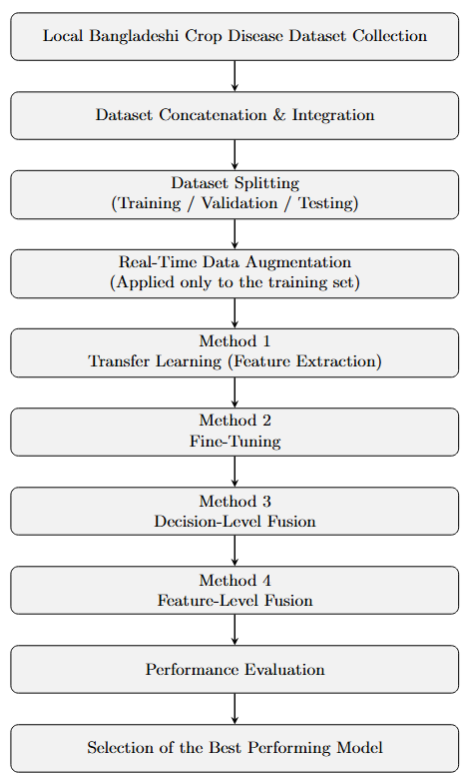
\includegraphics[width=0.6\textwidth]{img/Overall_Workflow.png} 
    \caption{Overall research workflow for the proposed crop disease detection system.}
    \label{fig:research_workflow} % Keep this label identical to your old code!
\end{figure}


\subsection{Dataset Collection}

One of the crucial factors for the effectiveness of deep learning models is the quality and variability of training data. As our focus is to design a crop disease detection model that is efficient in Bangladesh agricultural context, instead of solely relying on the commonly used PlantVillage dataset, we carefully chose publicly available crop disease datasets that are specific to our context, to ensure better generalizability in real-world scenario in Bangladeshi agriculture.

To assemble our dataset, we sourced images of crop diseases from publicly accessible platforms like Kaggle and Mendeley Data. Our assembled dataset include images of three economically important crops in Bangladesh – rice, potato and wheat – acquired from natural fields conditions.

The aforementioned datasets are selected because they feature an array of distinct disease classes, and include natural environment images and are labelled appropriately for use in deep learning based classification.

\begin{table}[H]
\centering
\begin{tabular}{|l|l|l|l|l|} 
\hline
\textbf{Dataset} & \textbf{Crop} & \textbf{Platform} & \textbf{Images} & \textbf{Environment} \\ \hline
Rice Leaf Diseases & Rice & Kaggle & $\sim$1,701 & Natural (BD) \\ \hline
Paddy Doctor & Rice & Kaggle & Subset & Mixed \\ \hline
Potato Leaf Disease & Potato & Mendeley & 3,076 & Uncontrolled \\ \hline
Wheat Disease & Wheat & Mendeley & 1,603 & Field (BD) \\ \hline
\end{tabular}
\caption{Overview of the source datasets used to compile the integrated training dataset.}
\label{tab:dataset_sources}
\end{table}


Rather than using a single dataset as it’s prevalent in the literature, in this study, multiple datasets of each crop are combined to form a single integrated dataset of varied disease conditions experienced by farmers in a practical environment. For each of the three target crops rice, potato and wheat exactly five distinct classes (including healthy and diseased states) were selected, resulting in a total of 15 classification categories. Irrelevant, highly similar, or underrepresented classes from the original sources were excluded. In summary, the integrated dataset comprises of about 6551 images classified into 15 classes and these images are ready for pre-processing, model training and evaluation steps.


\subsection{Dataset Integration}

% Explain concatenation
% Explain why PlantVillage was not used

Originally, all the collected datasets were acquired from separate public datasets with distinct directory structures, file names, and disease types. They were designed separately for different objectives so could not be used directly as a combined training data source to train a single deep learning model. The dataset integration stage combined these separate datasets into a single integrated dataset for comparative experimental comparisons. 
This created dataset contained 15 classes for 3 main crop types: potato, rice and wheat, with no specific divisions for training set, validation set, or testing set in this initial stage. 

To construct the unified dataset, a new root directory was created, and images from the selected rice, potato, and wheat datasets were reorganized according to their corresponding disease categories. Each disease category was placed into an individual class folder using a standardized naming convention, such as \texttt{potato\_early\_blight}, \texttt{rice\_blast}, and \texttt{wheat\_leaf\_blight}. This organization ensured that all crop species and disease classes followed a consistent folder hierarchy, allowing the dataset to be easily processed by TensorFlow's directory-based data loading utilities.

Images for all classes were pooled into the unified dataset. Splits were performed during the preprocessing phase later to make sure that all the experiment procedures used the same distribution of dataset.

\begin{figure}[H]
    \centering
    % Change 'workflow_screenshot.png' to whatever you name the file in your img folder
    % \textwidth makes it scale perfectly to the width of your page margins
    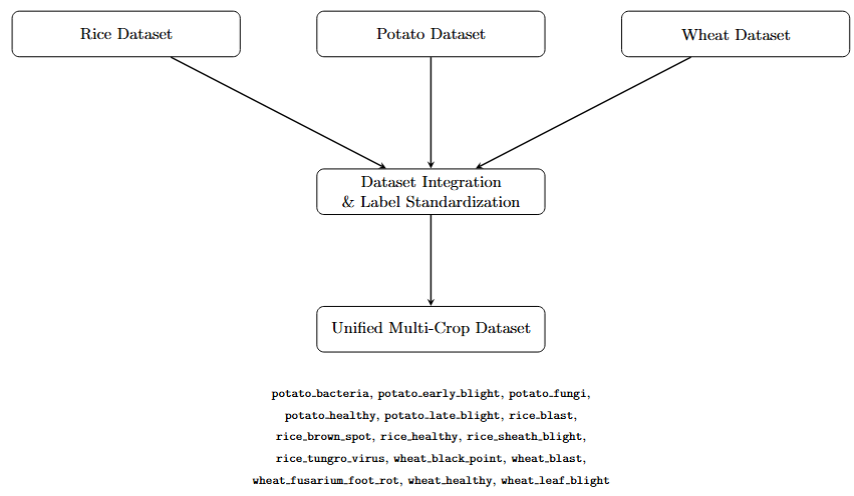
\includegraphics[width=0.85\textwidth]{img/Data_integration.png} 
   \caption{Dataset integration process from individual crop datasets into a unified multi-crop collection.}
    \label{fig:research_workflow} % Keep this label identical to your old code!
\end{figure}

The four individual datasets were merged into a single unified multi-crop repository. Classes with similar disease manifestations were standardized where possible, while preserving crop-specific distinctions. This integration created a more diverse and challenging dataset for training generalized models.

%%%FIGURE.............

\subsection{Data Preprocessing and Augmentation}

The integrated dataset then went through the complete preprocessing and augmentation process before feeding it to the model training process. This is performed so that all experimental approaches are trained and tested under exactly the same circumstances and so we are able to properly compare between the transfer learning and ensemble learning approaches tested in this study.

Following the dataset integration stage, consisting of \textbf{6,551} images across 15 disease classes, was partitioned into training, validation, and testing subsets using a \textbf{70\%-15\%-15\%} split ratio. Consequently, \textbf{4581} images were allocated to the training set, \textbf{978} images to the validation set, and \textbf{992} images to the testing set. Partitioning was done strata-wise for equal class distribution among subsets so that every disease category appeared at all experimental stage proportionaly.

Following dataset partitioning, all images underwent a unified preprocessing procedure before being supplied to the deep learning models. Since DenseNet121, MobileNetV2, and EfficientNetB0 require a fixed input resolution, every image was resized to \textbf{$224 \times 224$} pixels and processed using a batch size of 16. In contrast to traditional preprocessing pipelines where a single, global pixel normalization is applied before model inputs, the herein proposed pipeline left the pixel intensities of the data at the original levels within the data generator, letting the CNN models carry out their respective internal, model-specific preprocessing, hence perfectly fitting to the specific input needs of the different transfer learning models used.

To ensure the models generalize well to unseen images, thereby minimizing the possibility of over-fitting to the training images, real-time data augmentation was applied to the training dataset only by TensorFlow’s \texttt{ImageDataGenerator}. Instead of pre-generating and storing augmented images on disk, augmentation was applied to the images on-the-fly for every training epoch. This technique ensured a unique set of augmented images were encountered per epoch and reduced the required storage space. The training image dataset was augmented by random spatial and photometric transformations to mimic real-world agricultural field settings:

\begin{itemize}
\item Random rotations of up to $25^\circ$.
\item Horizontal and vertical translations of up to 15%.
\item Random zooming of up to 15%.
\item Shearing transformations of up to 10%.
\item Brightness variation between 80% and 120%.
\item Horizontal flipping with nearest-neighbor filling for newly created pixels.
\end{itemize}

Unlike the training dataset, both the validation and testing datasets remained completely unaugmented. This ensured that model performance was evaluated using unseen images without artificial modifications, providing an unbiased assessment of the models' generalization capability.

Finally, as the aggregated dataset had unequal numbers of images per disease category, we applied a class-weighting technique when training the model. The class weights were determined via Scikit-learn’s “balanced” approach (based on the number of samples per class), and this value was passed to the training procedure. Since under-represented classes receive a higher loss in backpropagation, the proposed methodology lessens bias to majority class, resulting in more consistent and less biased classification across all 15 classes.

% Image resizing
% Label encoding
% Train/Validation/Test split



\subsection{Transfer Learning (Feature Extraction)}

Transfer learning with feature extraction The first experimental setup for this work involved transfer learning with feature extraction. The pre-trained CNN models considered here were DenseNet121, MobileNetV2, and EfficientNetB0, used as the backbone architecture. The models were trained on ImageNet with 1000 classes and as we want to classify only 15 types of crops diseases, the original 1000-class classification layer was removed using \texttt{include\_top=False} and a new classifier was appended for the crop disease dataset of 15 classes. 

During this phase, all the weights of pre-trained backbone models were frozen. 



\begin{figure}[H]
    \centering
    % Change 'workflow_screenshot.png' to whatever you name the file in your img folder
    % \textwidth makes it scale perfectly to the width of your page margins
    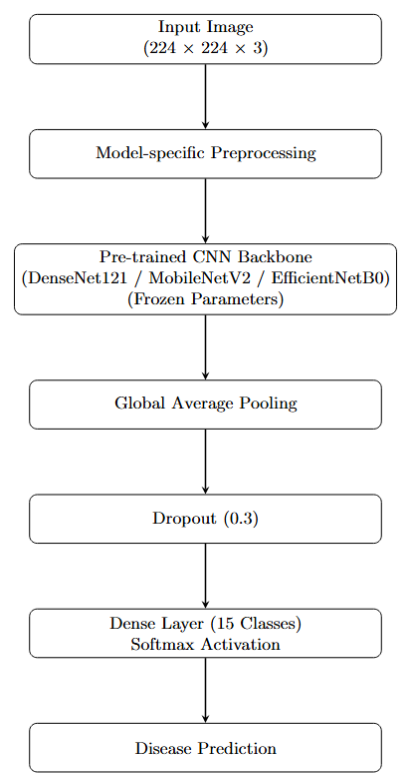
\includegraphics[width=0.65\textwidth]{img/Transfer_Learning.png} 
    \caption{Architecture of the Transfer Learning (Feature Extraction) pipeline.}
    \label{fig:research_workflow} % Keep this label identical to your old code!
\end{figure}

Only the weights of newly added classifier layers were trained. This classifier has a Global Average Pooling layer, a Dropout layer with dropout rate 0.3, and finally a Dense layer with 15 units and Softmax activation. For optimization, Adam was used with learning rate 0.001 and categorical cross-entropy as loss function. Early Stopping, Reduce Learning Rate on Plateau, and Model Checkpoint callbacks were used to monitor performance during training and to avoid overfitting. 

This experiment is performed to get the initial baseline score for each model before applying fine-tuning and ensemble.




% DenseNet
% MobileNet
% EfficientNet

\subsection{Fine-Tuning}

Post feature extraction stage A fine-tuning strategy was used to enhance the performances of the pre-trained CNN models. The previously trained DenseNet121, MobileNetV2, and EfficientNetB0 models were loaded. The convolutional backbone of each pre-trained model was partially unfrozen to be further trained on the joint crop disease data.

Only the upper layers of each backbone model were unfrozen while the previous lower layers remained frozen. It means the model adjusted its higher-level feature extraction capabilities on local crop disease images rather than completely retraining the whole network, so the general visual features gained on ImageNet are kept.
The models were recompiled with Adam optimizer and an extremely small learning rate of $1 \times 10^{-5}$. The models were then re-trained for several epochs with the same training/validation set split and class weight configuration used in the feature extraction phase. Model Checkpoint, Early Stopping, and Reduce Learning Rate on Plateau methods were once more employed to obtain the best performance.


\begin{figure}[H]
    \centering
    % Change 'workflow_screenshot.png' to whatever you name the file in your img folder
    % \textwidth makes it scale perfectly to the width of your page margins
    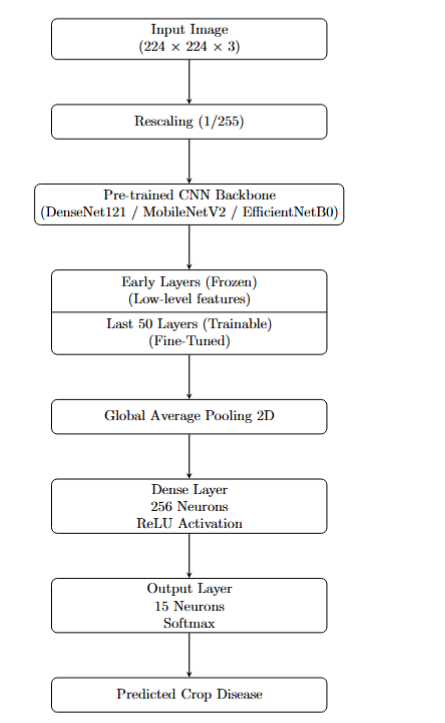
\includegraphics[width=0.65\textwidth]{img/Fine_tuning.png} 
   \caption{Architecture of the Fine-Tuning approach.}
    \label{fig:research_workflow} % Keep this label identical to your old code!
\end{figure}

This stage's purpose was to explore if partially training pre-trained backbones improves the classification performance compared to the feature extraction phase, prior to the proposal of feature-level and decision-level fusion methods.






% Explain unfreezing
% Small learning rate
\subsection{Decision-Level Fusion}

For enhance classification performance in overall. A Decision-Level Fusion method was introduced by combine all of the knowledge of the three CNNs fined-tune model(DenseNet121, MobileNetV2, EfficientNetB0) knowledge. Instead of a single model, the presented architecture utilize of prediction output of all three expert networks to make a final prediction. 

The three fine-tuned models were first loaded and their weights were frozen to preserve the knowledge acquired during the previous training stage. A unified input layer was then created, where model-specific preprocessing was applied internally. The processed inputs were simultaneously forwarded to the three expert networks, producing prediction vectors for each model.

Next, all prediction vectors from three backbone model were concatenated in to one feature presentation and feed into Dense layer with 64 neurons with relu activation, and then applied Dropout layer with 0.2 and finally Softmax layer with 15 neurons outputted the prediction disease. During training, Adam optimizer and categorical cross-entropy loss function were used with all backbone models frozen, except only the new added fusion classifier layer was optimized.

Our goal is to make full use of the different specialties of three CNNs architectures and improve the classification accuracy better than single transfer learning and fined-tuned models.

\begin{figure}[H]
    \centering
    % Change 'workflow_screenshot.png' to whatever you name the file in your img folder
    % \textwidth makes it scale perfectly to the width of your page margins
    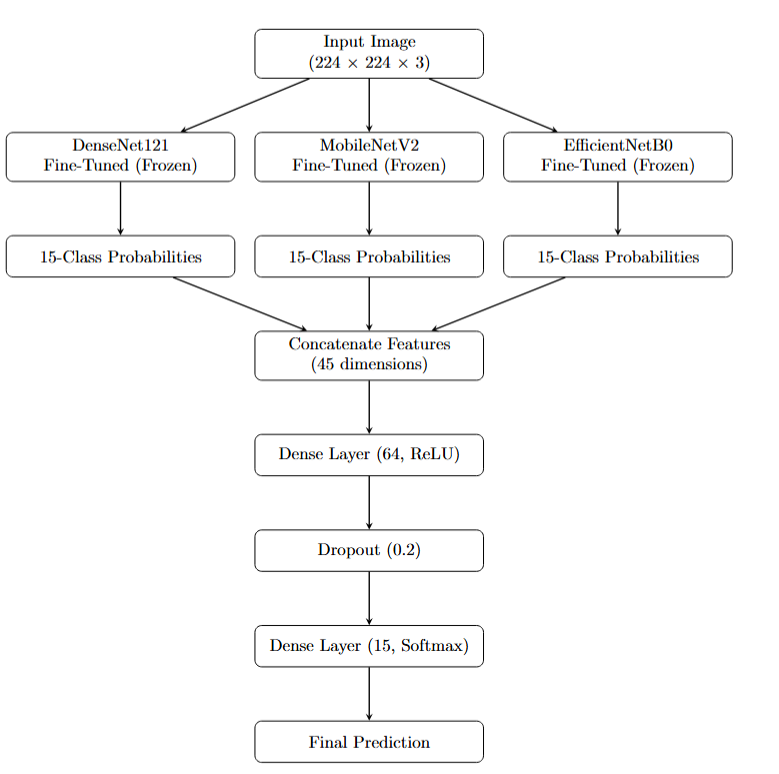
\includegraphics[width=0.75\textwidth  height=15cm, keepaspectratio]{img/Decision_level_Arc.png} 
    \label{fig:research_workflow} % Keep this label identical to your old code!
    \caption{Decision-Level Fusion architecture combining multiple CNN backbones.}
\end{figure}



% Meta learner architecture
% Diagram

\subsection{Feature-Level Fusion}

To further improve the classification performance, a feature-level fusion approach was proposed by combining the deep feature representations extracted from the three fine-tuned CNN models: DenseNet121, MobileNetV2, and EfficientNetB0. In this approach, instead of the direct prediction scores, we chose to directly feed the extracted high level feature vectors from each backbone.

Initially, three of the fine-tuned models (those with modified feature extraction layers) were utilized to extract deep feature representations for each of the images from the training and validation sets. These representations were cached on disk so that they did not have to be recalculated with each subsequent run of training, minimizing compute time and GPU RAM consumption. The features from the models were of different sizes; these were compressed into a unified 256-dimensional feature vector via fully connected layers. 

Thus, the 1024-dimensional features from DenseNet121, and the 1280-dimensional features from MobileNetV2 and EfficientNetB0, were all down-sampled to 256. 

After each such layer, batch normalization, a ReLU activation function and Dropout were used to stabilize the features and prevent over-fitting.

\begin{figure}[H]
    \centering
    % You can adjust the 8cm to whatever height looks best.
    % keepaspectratio prevents the image from looking stretched or squished!
    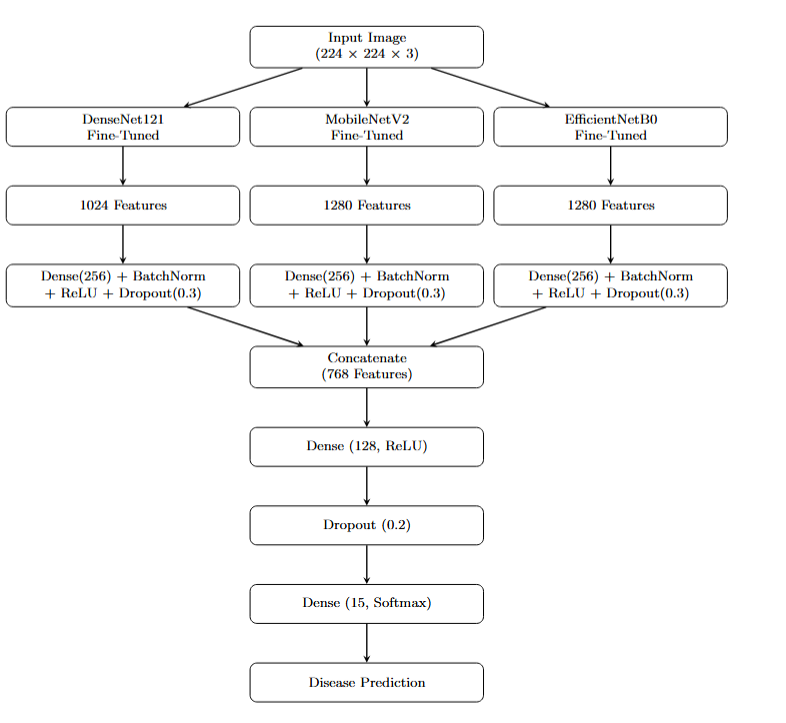
\includegraphics[width=0.85\textwidth, height=15cm, keepaspectratio]{img/Feature_level_Arc.png} 
    \caption{Feature-Level Fusion architecture with individual dense heads before concatenation.}
    \label{fig:feature_level_fusion} 
\end{figure}

Finally, the three compressed feature vectors were concatenated into a 768-dimensional feature representation that was fed into the last fusion classifier. This fusion classifier was composed of a Dense layer with 128 neurons followed by a Dropout layer and a Softmax output layer with 15 neurons, which represent the disease classes. The entire fusion classifier was trained with Adam optimizer using categorical cross-entropy loss, whereas the feature extraction networks are not updated.

The goal of this approach was to leverage the complementary feature representations captured by the three CNN architectures to obtain a more discriminative feature space for crop disease classification. 

Feature-level fusion combines deep features extracted from multiple fine-tuned CNN backbones before the final classification head. The architecture is shown below:




% 768-feature architecture
% Diagram

%------------------------------------------------


% Large workflow diagram
% 768-feature architecture
% Diagram

%------------------------------------------------

\section{Tools and Technologies Used}

The proposed crop disease detection system was developed using several software tools, programming libraries, and hardware resources. These technologies were utilized throughout the stages of dataset preprocessing, model training, evaluation, and visualization. Table~\ref{tab:tools_technologies} summarizes the major tools and technologies used in this research.

\begin{table}[H]
\centering

\label{tab:tools_technologies}
\begin{tabular}{|p{4cm}|p{10cm}|}
\hline
\textbf{Tool / Technology} & \textbf{Purpose} \\ \hline
Python 3.10 & Primary programming language used for model development and experimentation. \\ \hline
TensorFlow & Deep learning framework used for model training, fine-tuning, and inference. \\ \hline
Keras API & High-level API of TensorFlow used for constructing and training CNN models. \\ \hline
NumPy & Numerical computations and array manipulation. \\ \hline
Scikit-learn & Dataset utilities, class weight computation, and performance evaluation metrics. \\ \hline
Matplotlib & Visualization of training curves and experimental results. \\ \hline
Seaborn & Generation of confusion matrix heatmaps. \\ \hline
OpenCV & Image processing and manipulation during experimentation. \\ \hline
Visual Studio Code & Integrated Development Environment (IDE) used for implementation. \\ \hline
CUDA & GPU acceleration for deep learning model training. \\ \hline
cuDNN & GPU-optimized deep learning library used with TensorFlow. \\ \hline
\end{tabular}
\caption{Tools and Technologies Used}
\end{table}

The experiments were conducted on a personal computer equipped with an AMD Ryzen 5 5600H processor, 8 GB RAM, and an NVIDIA GeForce GTX 1650 GPU with 4 GB dedicated graphics memory. This hardware configuration provided sufficient computational capability for training and evaluating the proposed deep learning models.
% Python
% TensorFlow
% Keras
% VS Code
% HP Victus
% NVIDIA GTX 4GB
% CUDA
% OpenCV
% NumPy
% Pandas
% Matplotlib

%------------------------------------------------

\section{Work Division and Team Management}

The development of the proposed system was distributed among the three team members to ensure efficient execution across all phases of the project. Table \ref{tab:work_division} summarizes the core responsibilities assigned to each member.


\begin{table}[H]
\centering
\label{tab:work_division}
\renewcommand{\arraystretch}{1.3}
\begin{tabular}{|p{5.5cm}|c|c|c|}
\hline
\textbf{Task} & \textbf{Md. Shihab PK} & \textbf{Md. Shohan Uzzaman} & \textbf{Md. Sohel Rana} \\
\hline
Literature Review & \checkmark & \checkmark & \checkmark \\
\hline
Dataset Collection and Integration & & \checkmark & \checkmark \\
\hline
Data Preprocessing and Augmentation & & \checkmark & \checkmark \\
\hline
Transfer Learning Model Development & \checkmark & & \\
\hline
Fine-Tuning of CNN Models & \checkmark & & \\
\hline
Decision-Level Fusion Development & \checkmark & & \\
\hline
Feature-Level Fusion Development & \checkmark & & \\
\hline
Model Evaluation and Performance Analysis & \checkmark & \checkmark & \\
\hline
User Interface and Application Integration & & & \checkmark \\
\hline
Result Analysis and Discussion & \checkmark & \checkmark & \checkmark \\
\hline
Thesis Writing and Documentation & \checkmark & \checkmark & \checkmark \\
\hline
Final Review and Presentation Preparation & \checkmark & \checkmark & \checkmark \\
\hline
\end{tabular}
\caption{Work Division Among Team Members}
\end{table}
% Table

%------------------------------------------------

\section{Time Frame}

To ensure a structured and timely progression of the thesis, the project was divided into distinct developmental phases. Table \ref{tab:time_frame} illustrates the schedule, highlighting the major milestones achieved over the course of the final academic year.

\begin{table}[H]
\centering
\label{tab:time_frame}
\renewcommand{\arraystretch}{1.4}
\begin{tabular}{@{} l l @{}}
\toprule
\textbf{Project Phase \& Major Tasks} & \textbf{Completion Window} \\
\midrule
\textbf{Phase 1: Research \& Preparation} & \\
\hspace{0.5cm} Literature Review \& Requirement Analysis & September 2025 -- October 2025 \\
\hspace{0.5cm} Dataset Collection \& Image Preprocessing & November 2025 -- December 2025 \\
\midrule
\textbf{Phase 2: Core Development} & \\
\hspace{0.5cm} Base Model Training \& Fine-Tuning & January 2026 -- February 2026 \\
\hspace{0.5cm} Decision-Level \& Feature-Level Fusion & March 2026 -- April 2026 \\
\midrule
\textbf{Phase 3: Integration \& Finalization} & \\
\hspace{0.5cm} Application Integration \& System Testing & April 2026 -- May 2026 \\
\hspace{0.5cm} Model Evaluation \& Thesis Documentation & May 2026 -- June 2026 \\
\bottomrule
\end{tabular}
\caption{Project Time Frame and Major Milestones}
\end{table}
% Gantt Chart

%------------------------------------------------

\section{Summary}

In this chapter, we provided the detailed process and architectural design employed to produce the AI-based crop disease identification system. The research methodology commenced with detailed requirements gathering and a thorough analysis conducted to cater for functional and non-functional attributes to make the system useful in the real world. An inclusive and targeted image data of 6,551, capturing 15 types of plant diseases(including healthy) and three crops namely wheat, potato, and rice, was gathered and properly organized. After gathering, it was fused and meticulously pre-processed with the use of real-time image enhancement, on-the-fly image augmentation, and balancing classes.

The chapter then outlined the progressive deep learning strategies employed, transitioning from baseline feature extraction using DenseNet121, MobileNetV2, and EfficientNetB0, to targeted fine-tuning. Building upon these base models, two advanced ensemble architectures were detailed: a weighted decision-level fusion utilizing prediction vectors, and a highly discriminative feature-level fusion synthesizing deep morphological features. Finally, the hardware, software tools, team work division, and chronological milestones were documented to provide a transparent overview of the project's execution. With the methodological framework established.
\chapter{Implementation and Results}
This chapter details the experimental setup and evaluates the performance of multiple deep learning architectures applied to the localized crop disease dataset. It provides the progression from initial transfer learning and fine-tuning to an enriched fusion approach, culminating in a comparative performance analysis across all the tested architectures.

\section{Environment Setup}
All experiments presented in this study were conducted on the same hardware and software platform to ensure consistency and reproducibility throughout the model development and evaluation process.

The proposed crop disease detection system was implemented using the Python programming language with the TensorFlow deep learning framework and its Keras API. Visual Studio Code (VS Code), utilizing Jupyter Notebooks (\texttt{.ipynb}), was used as the primary development environment for model implementation, training, and testing. Image preprocessing and augmentation were performed using TensorFlow's \texttt{ImageDataGenerator}, while NumPy was utilized for numerical computations and data manipulation.

The experiments were executed on an HP Victus 16 laptop equipped with an AMD Ryzen 5 5600H processor, 8 GB RAM, and an NVIDIA GeForce GTX 1650 GPU with 4 GB dedicated graphics memory. GPU acceleration was utilized during the training process to reduce computational time for deep learning model optimization.

Table \ref{tab:environment} summarizes the hardware and software configuration used throughout the experiments.

\begin{table}[H]
\centering
\begin{tabular}{|l|l|}
\hline
\textbf{Component} & \textbf{Specification} \\ \hline
Operating System & Windows 11 \\ \hline
Development Environment & VS Code (Jupyter Notebooks) \\ \hline
Programming Language & Python \\ \hline
Deep Learning Framework & TensorFlow (Keras API) \\ \hline
Image Processing & TensorFlow ImageDataGenerator \\ \hline
Scientific Computing & NumPy \\ \hline
Visualization & Matplotlib \\ \hline
Processor & AMD Ryzen 5 5600H \\ \hline
Memory (RAM) & 8 GB \\ \hline
Graphics Processing Unit & NVIDIA GeForce GTX 1650 (4 GB) \\ \hline
\end{tabular}
\caption{System specifications used for model training and evaluation.}
\label{tab:environment}
\end{table}

\section{Testing and Evaluation}
\subsection{Test Dataset}
Following the entire training procedure, the produced models were tested using the identical reserved test image data set containing \textbf{992} unseen images. It is noteworthy that this test set was completely independent of the training and validation data during data segmentation and was not used for training the models or hyperparameter optimisation. No data augmentation or artificial transformations were introduced to the images in the test set to ensure that their evaluation indicated how well the trained models can generalize to unseen images. Having a uniform test data set among all methods ensures a reliable and objective evaluation of the transfer learning, fine-tuning, decision level fusion and feature level fusion strategies.

\subsection{Evaluation Metrics}

The performance of each proposed model was evaluated using several standard classification metrics. Since crop disease identification is a multi-class classification problem, multiple evaluation criteria were considered to provide a comprehensive assessment of model performance.

\subsubsection{Accuracy:}

Accuracy measures the overall proportion of correctly classified samples among all test samples.

\begin{equation}
Accuracy = \frac{TP + TN}{TP + TN + FP + FN}
\end{equation}

where $TP$, $TN$, $FP$, and $FN$ denote the number of true positives, true negatives, false positives, and false negatives, respectively.

\subsubsection{Precision:}

Precision measures how many samples predicted as a particular disease actually belong to that disease class.

\begin{equation}
Precision = \frac{TP}{TP + FP}
\end{equation}

Higher precision indicates fewer false positive predictions.

\subsubsection{Recall:}

Recall evaluates how effectively the model identifies all samples belonging to a particular disease class.

\begin{equation}
Recall = \frac{TP}{TP + FN}
\end{equation}

A higher recall indicates fewer missed disease cases.

\subsubsection{F1-Score:}

The F1-score is the harmonic mean of Precision and Recall, providing a balanced evaluation when class distributions are uneven.

\begin{equation}
F1 = \frac{2 \times Precision \times Recall}{Precision + Recall}
\end{equation}

\subsubsection{Confusion Matrix:}

For more thorough evaluation of classification performance, a confusion matrix was also created for each experimental model. A confusion matrix clearly indicates the association between real class of the disease and its corresponding predicted class. By observing the matrix, we can clearly differentiate between correct classifications and common errors or confusion between different diseases.



\section{Results and Discussion}
This section presents the experimental results obtained from the four proposed methodologies. All models were trained using the same preprocessing pipeline and evaluated on the identical unseen test dataset to ensure a fair comparison. The performance of each method is presented individually, followed by an overall comparative analysis to determine the most effective architecture for Bangladeshi crop disease classification.

%------------------------------------------------

\subsection{Method 1: Transfer Learning (Feature Extraction)}

The first experiment evaluated the performance of transfer learning using the feature extraction strategy. Three pre-trained CNN architectures, namely DenseNet121, MobileNetV2, and EfficientNetB0, were employed as fixed feature extractors. During this stage, the convolutional backbone of each model remained frozen, while only the newly added classification head was trained on the integrated crop disease dataset.

Table \ref{tab:feature_extraction_results} summarizes the overall classification performance of the three backbone models on the unseen test dataset.
\begin{table}[H]
\centering
\label{tab:feature_extraction_results}
\begin{tabular}{lcccc}
\hline
\textbf{Model} & \textbf{Accuracy (\%)} & \textbf{Precision} & \textbf{Recall} & \textbf{F1-score} \\
\hline
DenseNet121    & 90.93 & 0.91 & 0.91 & 0.91 \\
MobileNetV2    & 89.92 & 0.90 & 0.90 & 0.90 \\
EfficientNetB0 & \textbf{92.44} & \textbf{0.93} & \textbf{0.92} & \textbf{0.92} \\
\hline
\end{tabular}
\caption{Performance of Feature Extraction Models on the Test Dataset}
\end{table}


Among the three transfer learning models, EfficientNetB0 achieved the highest classification accuracy of 92.44\%, followed by DenseNet121 with 90.93\% and MobileNetV2 with 89.92\%. The results indicate that all three architectures were capable of learning meaningful crop disease representations despite training only the newly added classifier layers.

Overall, the feature extraction approach established a strong baseline for the subsequent fine-tuning and ensemble learning experiments.

% Architecture figure (optional)
% Training curves (Accuracy & Loss)
% Confusion Matrix
% Classification Report
% Discussion

%------------------------------------------------

\subsection{Method 2: Fine-Tuning}

Following the feature extraction experiment, a fine-tuning strategy was applied to further improve the classification performance of the pre-trained CNN models. In this stage, the upper layers of DenseNet121, MobileNetV2, and EfficientNetB0 were partially unfrozen and trained using a smaller learning rate, allowing the models to adapt their high-level feature representations toward the characteristics of Bangladeshi crop disease images.

Table \ref{tab:finetuning_results} presents the performance comparison of the fine-tuned models on the unseen test dataset.

\begin{table}[H]
\centering
\label{tab:finetuning_results}
\begin{tabular}{lcccc}
\hline
\textbf{Model} & \textbf{Accuracy (\%)} & \textbf{Precision} & \textbf{Recall} & \textbf{F1-score} \\
\hline
DenseNet121 & 92.54 & 0.93 & 0.93 & 0.93 \\
MobileNetV2 & \textbf{93.65} & \textbf{0.94} & \textbf{0.95} & \textbf{0.94} \\
EfficientNetB0 & 93.15 & 0.94 & 0.93 & 0.93 \\
\hline
\end{tabular}
\caption{Performance of Fine-Tuned Models on the Test Dataset}
\end{table}

The fine-tuning strategy improved the performance of all three backbone architectures compared with the initial feature extraction approach. MobileNetV2 achieved the highest accuracy of 93.65\%, followed by EfficientNetB0 with 93.15\% and DenseNet121 with 92.54\%.

Compared with the feature extraction stage, DenseNet121 improved from 90.93\% to 92.54\%, MobileNetV2 improved from 89.92\% to 93.65\%, and EfficientNetB0 improved from 92.44\% to 93.15\%. These improvements indicate that allowing the higher-level convolutional layers to adapt to the local crop disease characteristics helped the models learn more discriminative features.

To provide a comprehensive overview of the architectural improvements, Figure \ref{fig:model_comparison} visualizes the performance trajectory of all six evaluated models. 

\begin{figure}[H]
\centering
% Replace 'Your_Image_Name.png' with your actual file path/name
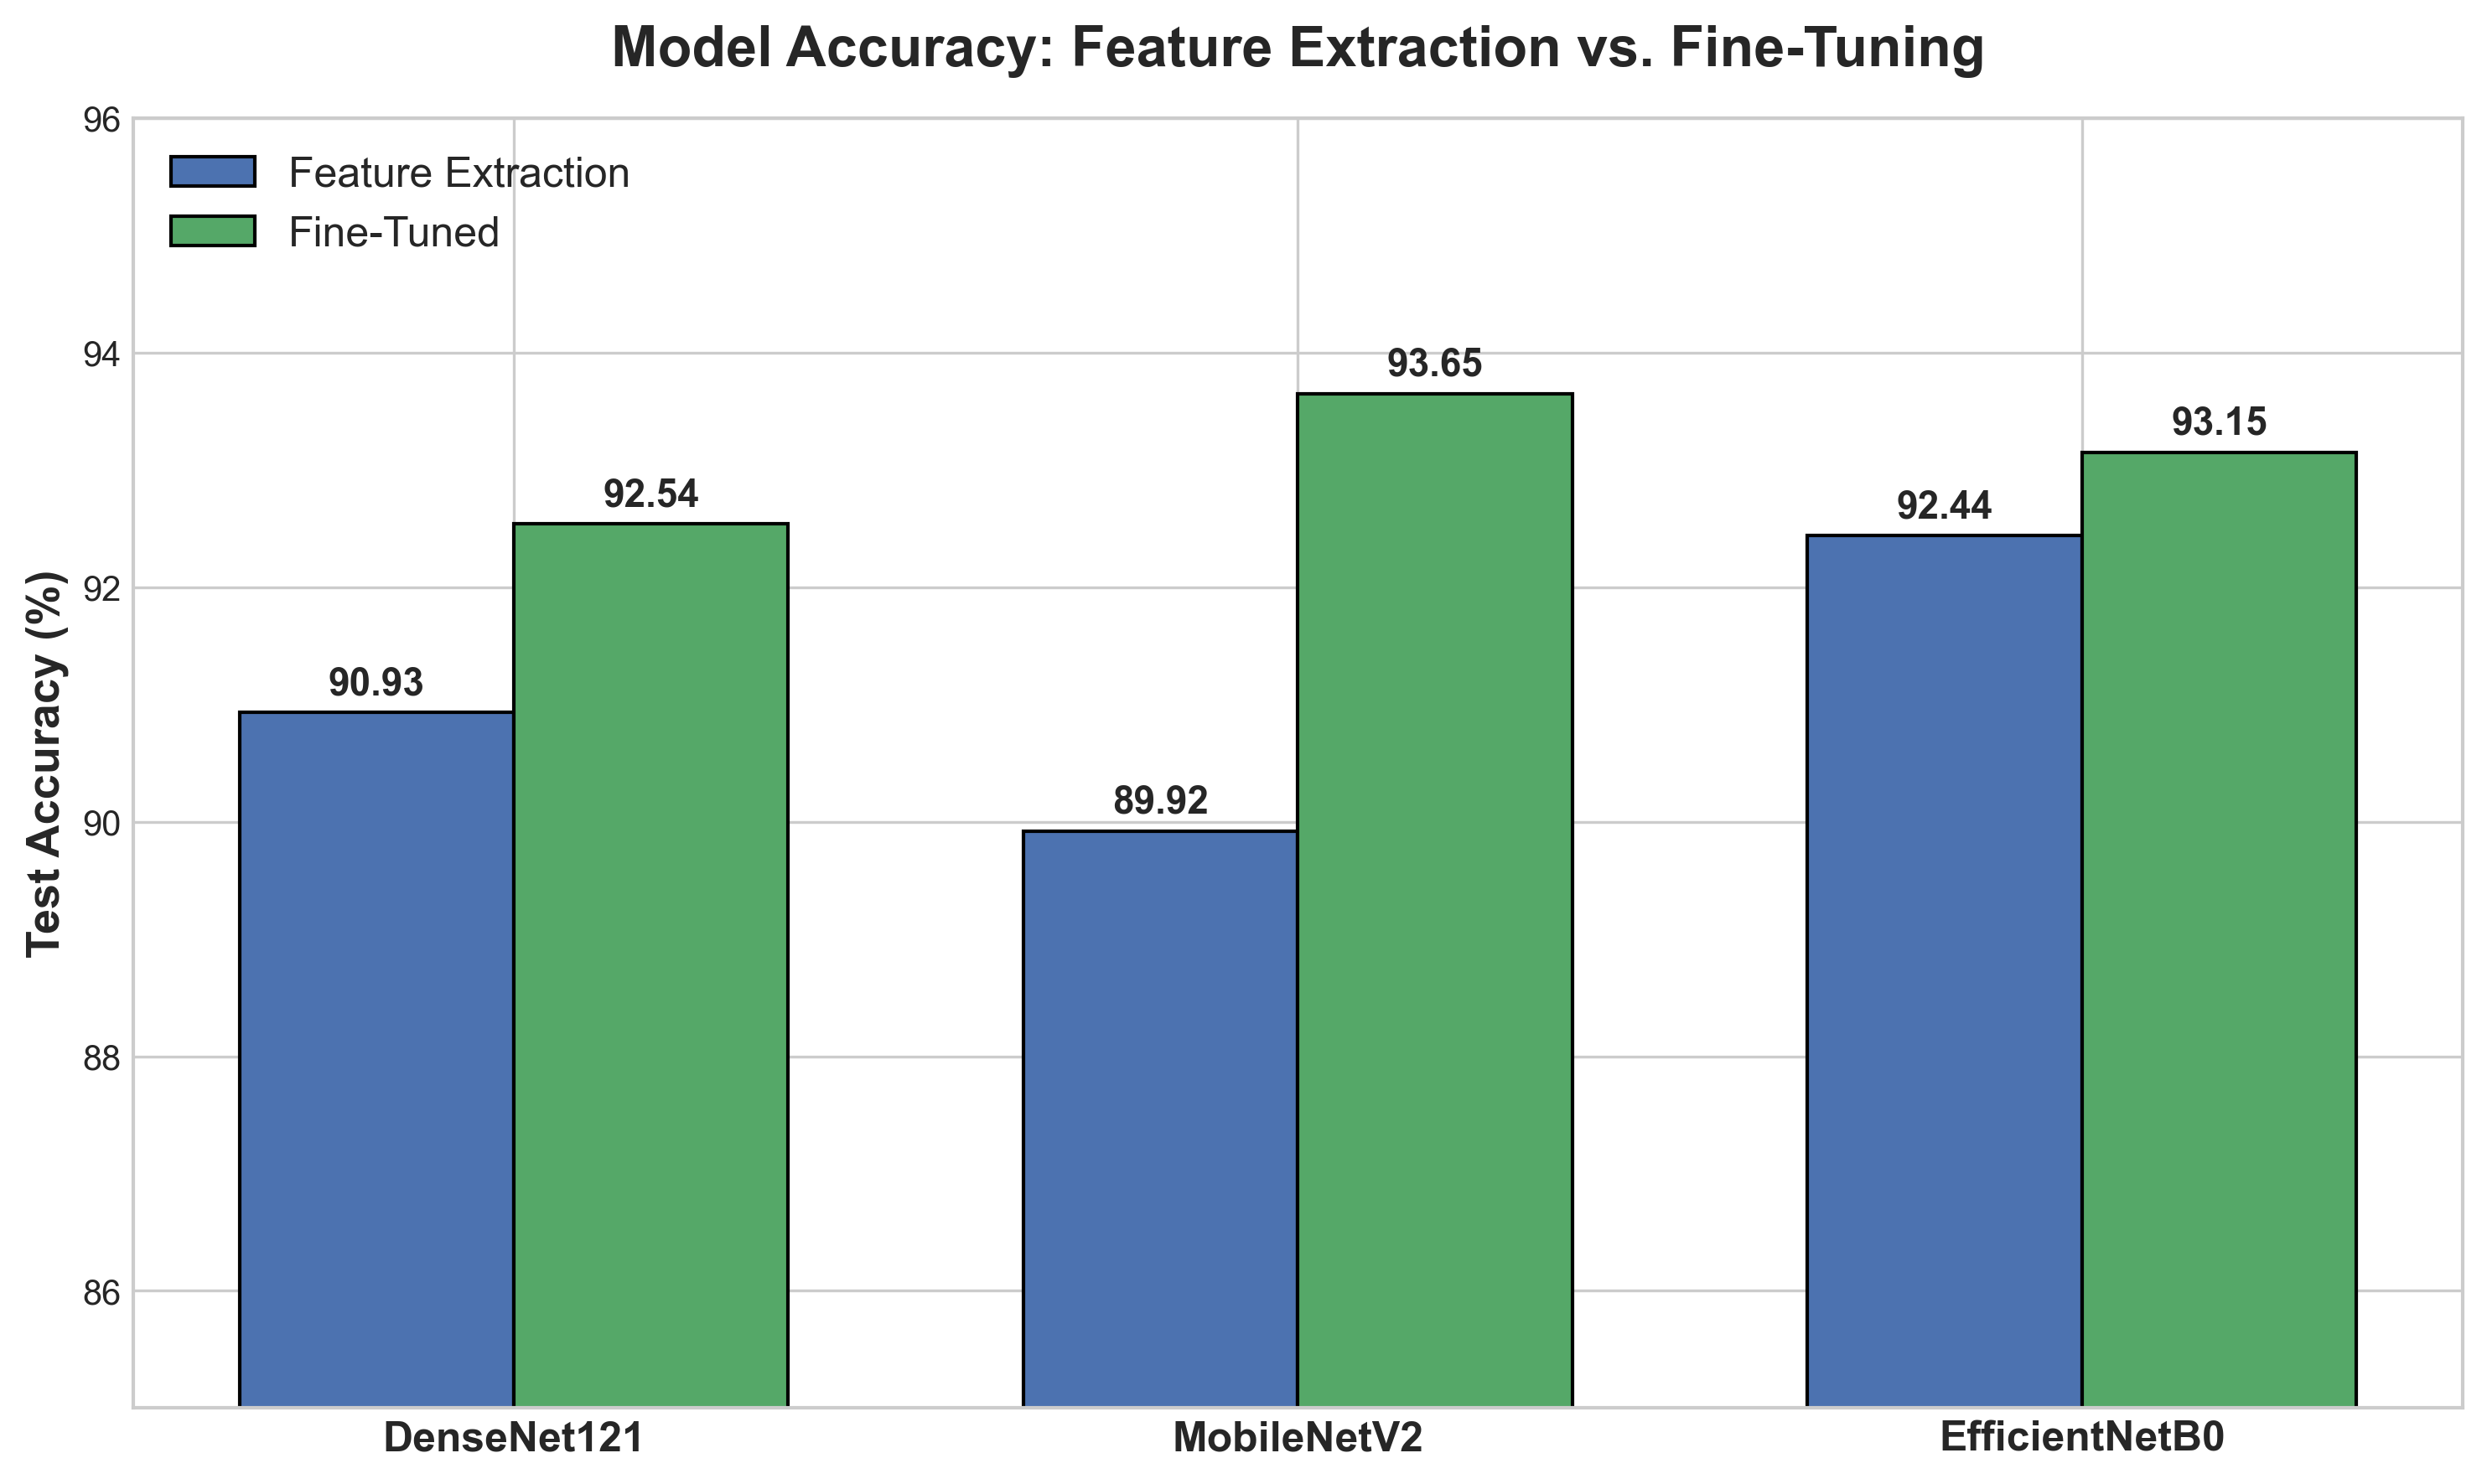
\includegraphics[width=0.85\textwidth]{img/Accuracy_Comparison_Bar_Chart.png} 
\caption{Performance comparison of all six models (Feature Extraction vs. Fine-Tuning) evaluated on the unseen test dataset.}
\label{fig:model_comparison}
\end{figure}

However, as feature extractors, EfficientNetB0 gave the highest result, while MobileNetV2 recorded the most substantial improvement post fine-tuning. This implied that the effectiveness of a pre-trained model to transfer generic features from ImageNet is not the ultimate determinant of performance over a specialized dataset of a certain domain. Through Fine-Tuning the model can capture the distinctive visual features of specific crop diseases within the context of Bangladeshi region.

In a general aspect, the fine tuning of this experimental model proved that a proper transfer based adaptation leads to better classification of disease from data-set, whereas directly taking an as feature classifier out perform by the fine tuned model.
% Training curves
% Confusion Matrix
% Classification Report
% Discussion

%------------------------------------------------

\subsection{Method 3: Decision-Level Fusion}

In order to investigate if the combination of various architectural choices could further increase predictability, a decision-level fusion ensemble was implemented. Unlike simple probability averaging, this method utilized a dynamically weighted learning approach. The ensemble was designed to learn which individual base model produced the most reliable predictions for specific disease categories, adjusting the classification weights accordingly to prioritize the strongest model for any given input class.

Table \ref{tab:fusion_results} summarizes the performance metrics of the fusion model on the unseen test dataset.

\begin{table}[H]
\centering
\label{tab:fusion_results}
\renewcommand{\arraystretch}{1.2}
\begin{tabular}{lcccc}
\hline
\textbf{Model} & \textbf{Accuracy (\%)} & \textbf{Precision} & \textbf{Recall} & \textbf{F1-score} \\
\hline
Decision-Level Fusion & 91.23 & 0.92 & 0.91 & 0.91 \\
\hline
\end{tabular}
\caption{Performance of the Decision-Level Fusion Model on the Test Dataset}
\end{table}

Interestingly, despite this targeted weighting approach, the decision-level fusion model achieved an overall accuracy of 91.23\%. While this established a highly capable classification threshold, it did not surpass the peak performance of the individual fine-tuned models. 

This performance dynamic suggests that learning class-specific model weights at the final decision layer likely led to overfitting during the ensemble's training phase. By rigidly prioritizing specific models for specific diseases based on training patterns, the ensemble lost the generalization ability required for the high variance of the unseen test set. Rather than synergistically compensating for weaknesses, the weighted fusion ultimately diluted the robust, generalized confidence of the strongest individual networks.

To visualize exactly where the ensemble struggled with conflicting predictions, the confusion matrix for the Decision-Level Fusion model is presented in Figure \ref{fig:fusion_confusion}.

\begin{figure}[H]
\centering
% Update the path/filename if you placed it in an images folder
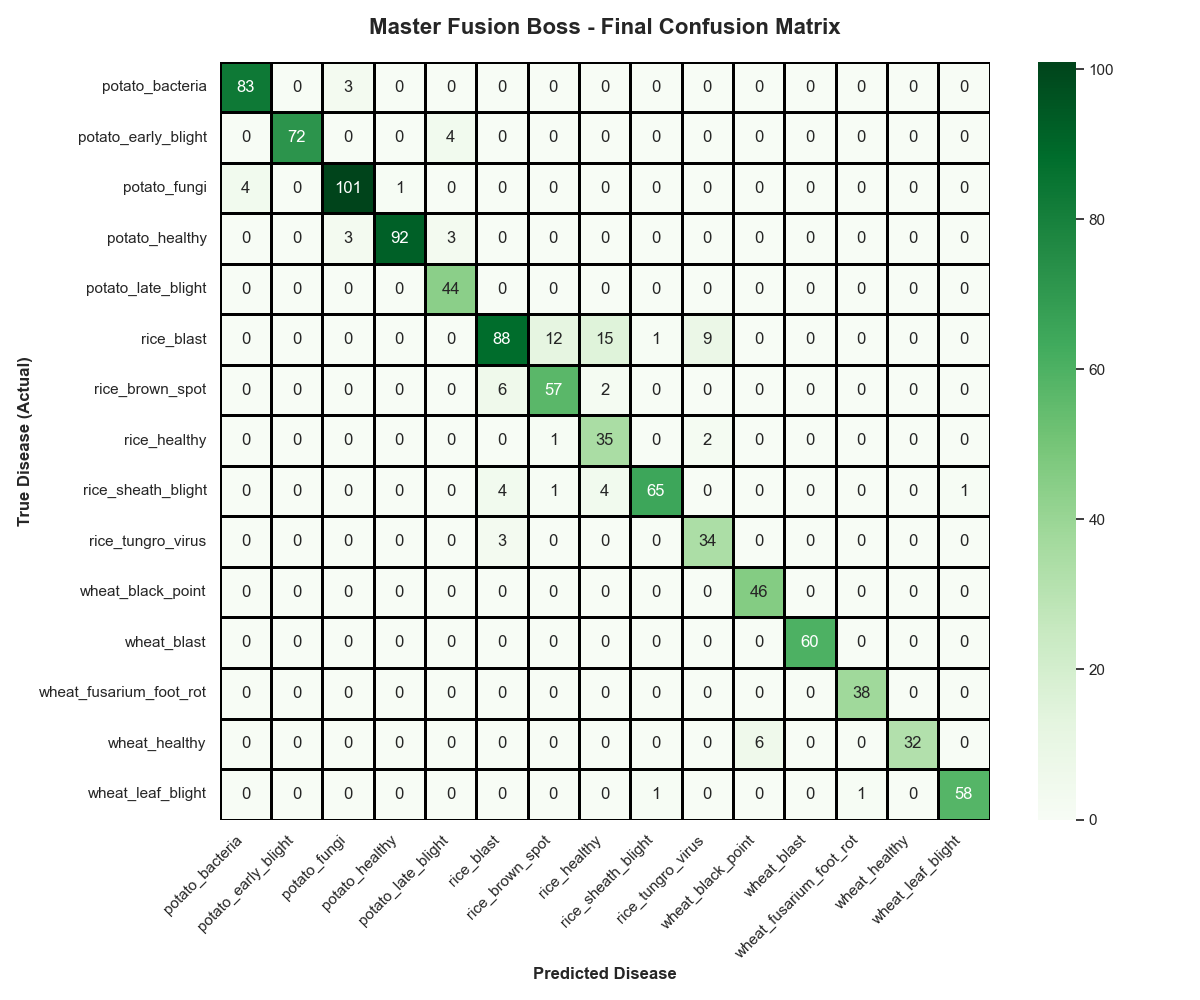
\includegraphics[width=0.85\textwidth]{img/Decision_Level__Fusion_Boss_Confusion_Matrix.png} 
\caption{Confusion matrix for the Decision-Level Fusion ensemble, illustrating class-specific prediction overlaps.}
\label{fig:fusion_confusion}
\end{figure}

The matrix clearly highlights the specific misclassifications that dragged down the ensemble's overall accuracy. For instance, the fusion model exhibited noticeable confusion between specific rice disease categories, which the standalone fine-tuned models had navigated more successfully. This visual breakdown reinforces the conclusion that complex, localized datasets benefit more from targeted fine-tuning than from weighted decision-level aggregation. Ultimately, the isolated, highly specialized MobileNetV2 (at 93.65\% accuracy) proved to be a more robust and computationally efficient option for this specific agricultural problem, demonstrating that a specialized standalone system can sometimes outperform a generalized ensemble.
% Architecture
% Training curves
% Confusion Matrix
% Classification Report
% Discussion

%------------------------------------------------


\subsection{Method 4: Feature-Level Fusion}

In order to address the shortcomings encountered by the weighted decision-level approach, a feature-level fusion architecture was developed. Instead of learning weights for final probability distributions, this approach extracted the deep, multi-dimensional feature maps from the fine-tuned convolutional backbones of DenseNet121, MobileNetV2, and EfficientNetB0. These distinct feature vectors were concatenated into a single, comprehensive representation and fed into a newly trained dense classification head. 

Table \ref{tab:feature_fusion_results} outlines the exceptional performance metrics achieved by this combined architecture.

\begin{table}[H]
\centering
\label{tab:feature_fusion_results}
\renewcommand{\arraystretch}{1.2}
\begin{tabular}{lcccc}
\hline
\textbf{Model} & \textbf{Accuracy (\%)} & \textbf{Precision} & \textbf{Recall} & \textbf{F1-score} \\
\hline
Feature-Level Fusion & \textbf{96.27} & \textbf{0.97} & \textbf{0.96} & \textbf{0.96} \\
\hline
\end{tabular}
\caption{Performance of the Feature-Level Fusion Model on the Test Dataset}
\end{table}

The feature-level fusion approach yielded the highest predictive accuracy of the entire study, reaching a peak of 96.27\%. This massive leap in performance conclusively demonstrates that the individual networks were identifying complementary morphological features—for example, one architecture specializing in textural anomalies while another focused on edge detection. By merging these internal representations directly, the final classifier was able to leverage a far richer feature space than any single model could provide.

Figure \ref{fig:feature_fusion_confusion} presents the confusion matrix for this final architecture.

\begin{figure}[H]
\centering
% Update the path/filename if you placed it in an images folder
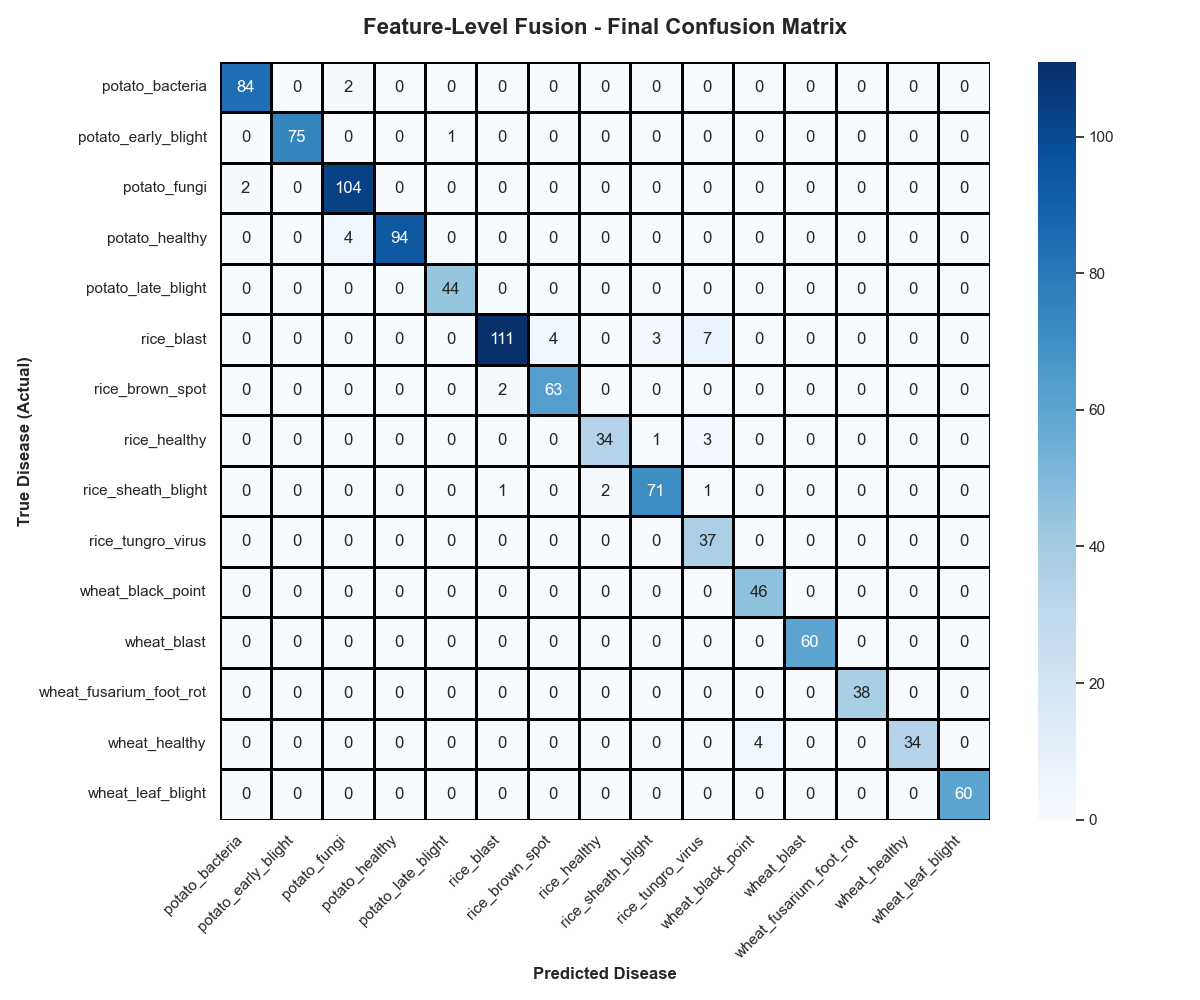
\includegraphics[width=0.85\textwidth]{img/Feature_Level_Fusion_Confusion_Matrix.png} 
\caption{Confusion matrix for the Feature-Level Fusion model, demonstrating highly accurate and distinct class separation.}
\label{fig:feature_fusion_confusion}
\end{figure}

The confusion matrix visually confirms the robustness of the feature-level fusion. The previously noted misclassifications in the decision-level ensemble—particularly the confusion between complex rice disease classes—were almost entirely resolved. Multiple classes, including \textit{wheat\_blast} and \textit{wheat\_fusarium\_foot\_rot}, achieved perfect classification (1.00 F1-score), solidifying this architecture as a highly reliable, deployment-ready solution for local agricultural settings.

% Architecture
% Training curves
% Confusion Matrix
% Classification Report
% Discussion

%------------------------------------------------

\subsection{Performance Comparison}

To comprehensively evaluate the progression of our architectural strategies, the optimal configurations from each experimental phase were compared. Table \ref{tab:master_comparison} presents the consolidated performance metrics for the fine-tuned base models alongside the two proposed ensemble techniques.

\begin{table}[H]
\centering

\label{tab:model_comparison}
\renewcommand{\arraystretch}{1.2}
\begin{tabular}{lcccc}
\hline
\textbf{Architecture} & \textbf{Accuracy (\%)} & \textbf{Precision} & \textbf{Recall} & \textbf{F1-score} \\
\hline
DenseNet121 (Fine-Tuned)    & 92.54 & 0.93 & 0.93 & 0.93 \\
EfficientNetB0 (Fine-Tuned) & 93.15 & 0.94 & 0.93 & 0.93 \\
MobileNetV2 (Fine-Tuned)    & 93.65 & 0.94 & 0.94 & 0.94 \\
Decision-Level Fusion       & 91.23 & 0.92 & 0.91 & 0.91 \\
\textbf{Feature-Level Fusion} & \textbf{96.27} & \textbf{0.97} & \textbf{0.96} & \textbf{0.96} \\
\hline
\end{tabular}
\caption{Master Performance Comparison of All Optimized Architectures}
\end{table}

The comparative analysis yields several critical insights into crop disease classification using local datasets. First, while individual lightweight models like MobileNetV2 perform exceptionally well (93.65\%) when properly fine-tuned, they possess inherent representational limits. Second, attempting to combine these models via a learned-weight decision-level fusion (91.23\%) proved detrimental. The ensemble likely overfitted its class-specific weights to the training data, losing generalization power on the test set and diluting overall predictive accuracy. 

To further contextualize these performance dynamics during the training phase, the accuracy and loss convergence histories for both ensemble approaches are presented in Figure \ref{fig:decision_history} and Figure \ref{fig:feature_history}.

\begin{figure}[H]
\centering
% Ensure the path matches where you store your images
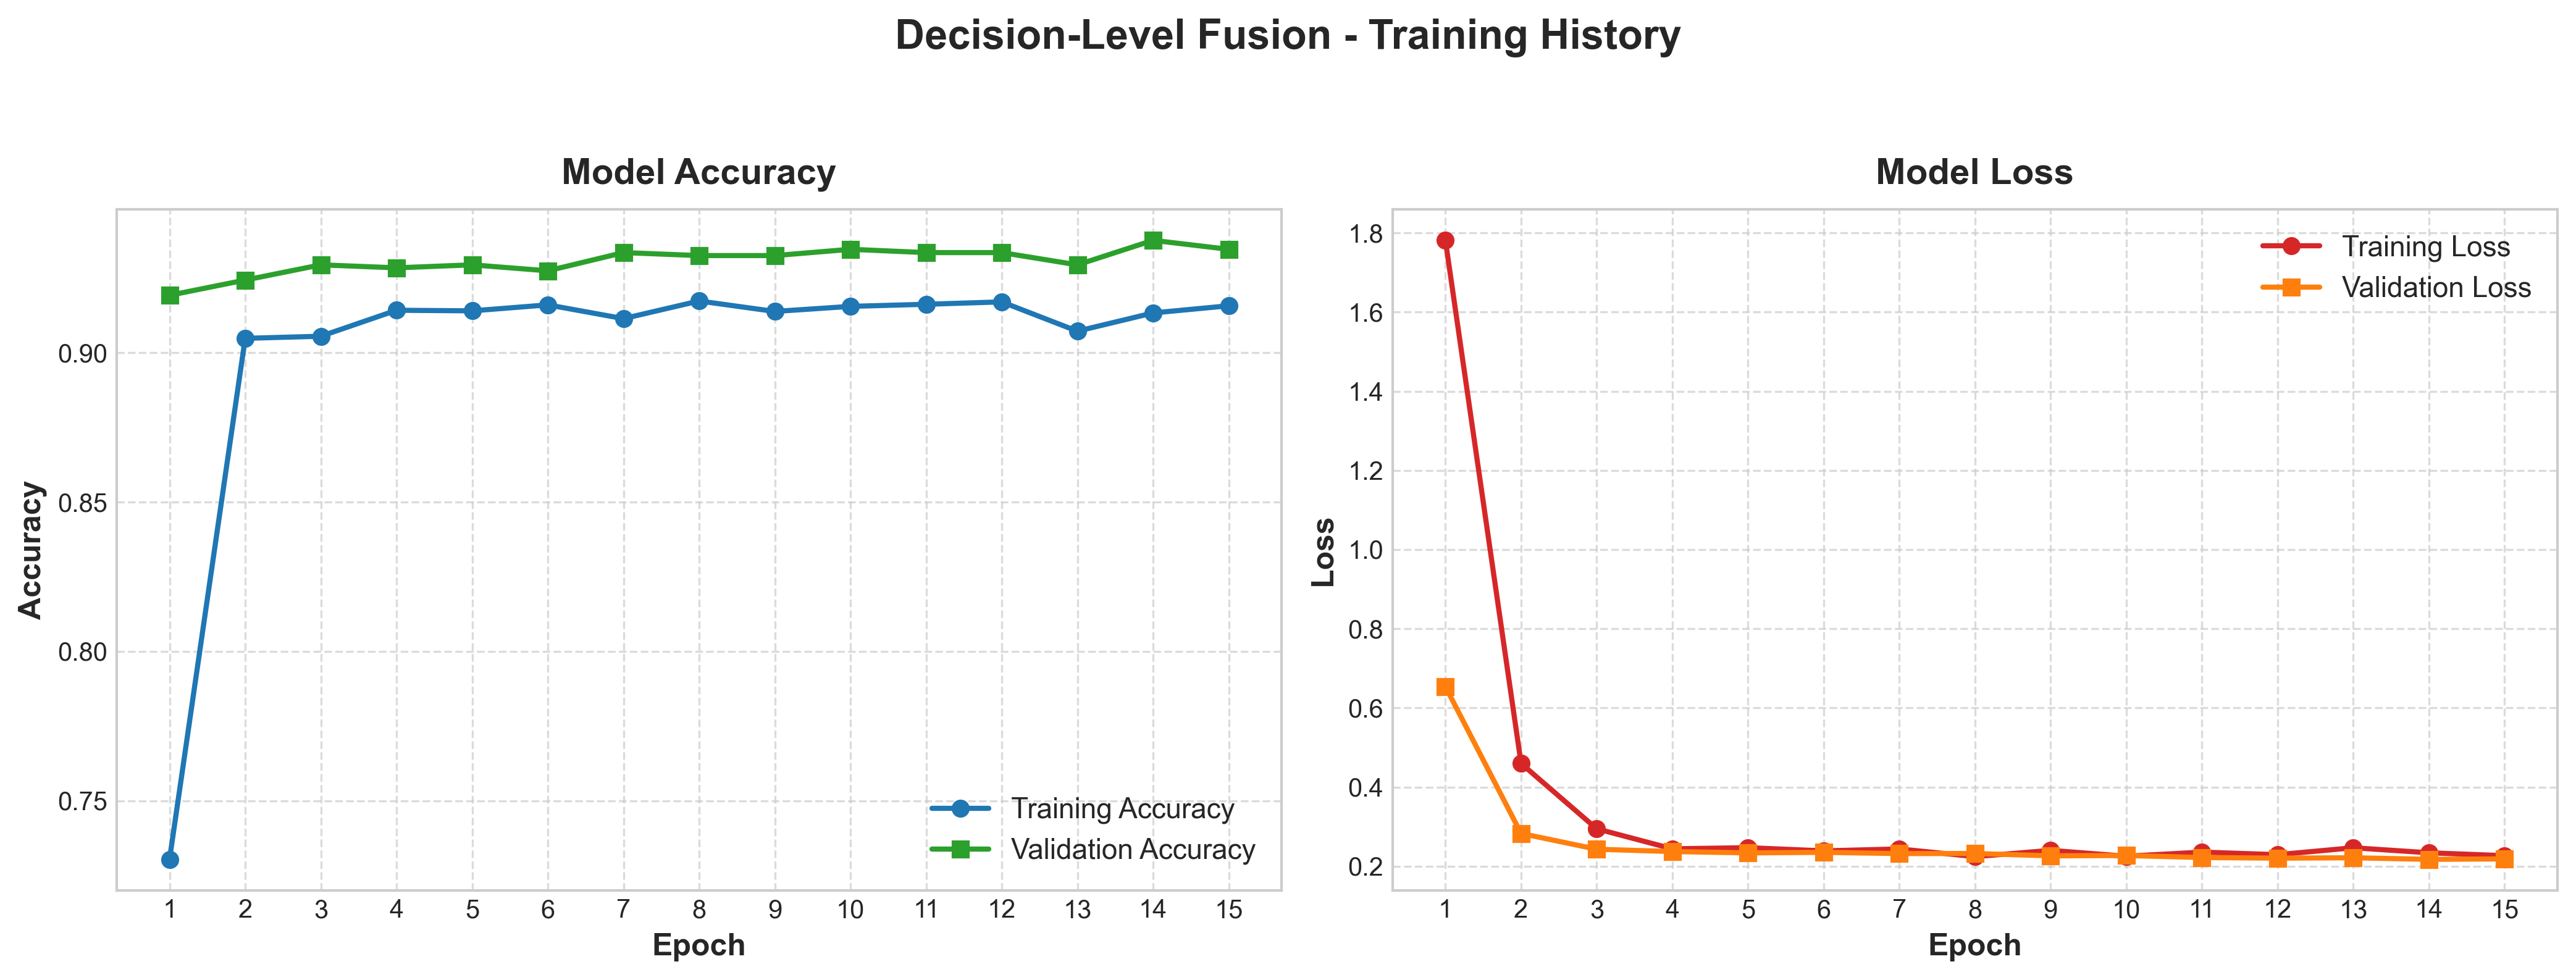
\includegraphics[width=0.95\textwidth]{img/Decision_Level_Training_History.png} 
\caption{Training and validation accuracy and loss history for the Decision-Level Fusion model.}
\label{fig:decision_history}
\end{figure}

\begin{figure}[H]
\centering
% Ensure the path matches where you store your images
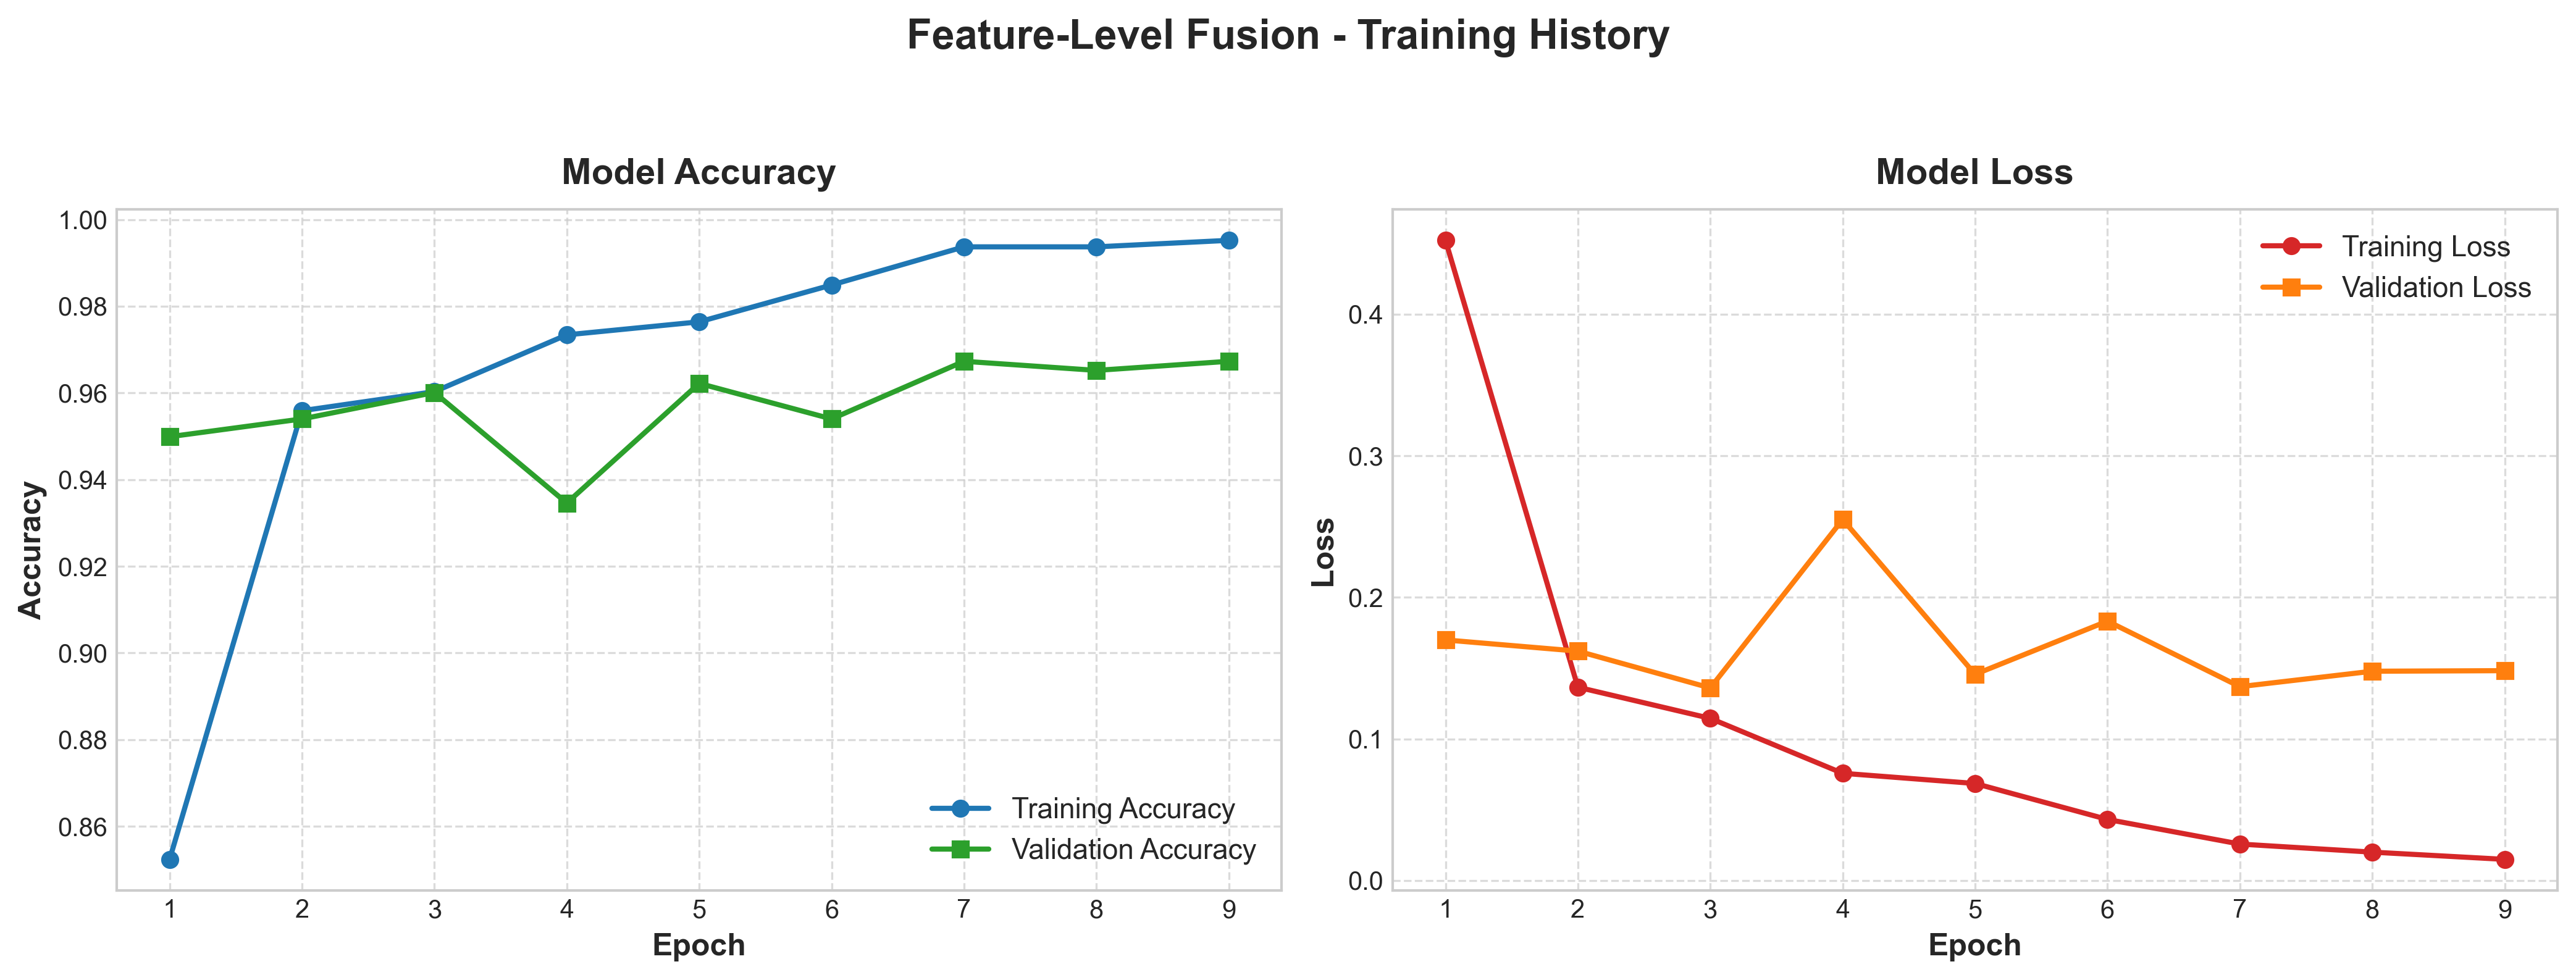
\includegraphics[width=0.95\textwidth]{img/Feature_Level_Training_History.png} 
\caption{Training and validation accuracy and loss history for the Feature-Level Fusion model.}
\label{fig:feature_history}
\end{figure}

Ultimately, the Feature-Level Fusion architecture emerged as the definitive solution, achieving a state-of-the-art accuracy of 96.27\%. By concatenating the deep feature maps of the individual networks before classification, the model successfully synthesized textural, spatial, and edge-based morphological data. This unified the proposed architecture proves that deep feature synthesis is highly effective at overcoming the high variance and real-world noise present in Bangladeshi agricultural environments.

% One comparison table

% Accuracy
% Precision
% Recall
% F1-score

% Bar chart (optional)

% Final discussion


\section{Summary}

The main findings of the experiments presented in this chapter to identify the optimal architecture for the crop disease detection problem on complex and local field dataset were outlined as follows:

1) Using individual lightweight models, a high performance standard was established using fine-tuned MobileNetV2 architecture (93.65\% accuracy), demonstrating that the effectiveness of general transfer learning approaches, though having limitation with inherent variability in real-life farm scenario. 

2) Using Decision Level Fusion approach (91.23\%) our effort to enhance the model robustness by creating class-dependent weight from the predicted probability vector of final classifier resulted over-fitting instead of supplementing weaknesses of base models. 

3) Feature Level Fusion architecture gave the best result, combining the deep internal feature representation of all the three base models via concatenation (compressing them with another compression layer) and training a final classifier resulted a maximum accuracy of 96.27\%. 

The conclusion derived is that for a highly variable and local field dataset, combining internal morphology features rather than combined prediction result achieved best accuracy. Hence, the proposed Feature Level Fusion model provide a state-of-the-art basis and robust model that can be implemented in real-life applications for crop disease detection in Bangladesh.
\chapter{Standards and Design Constraints}

This chapter outlines the industry standards, ethical considerations, and design constraints that guided the development of the AI-powered crop disease detection system. It also justifies the engineering complexity of the methodology and provides a cost-benefit analysis of the proposed solution.

\section{Compliance with the Standards}

To ensure the reproducibility, reliability, and maintainability of the proposed software pipeline, several industry-standard practices were adopted. 

\subsection{Software Standards}
The development of the deep learning models and data preprocessing pipelines strictly adhered to established software engineering protocols. 
\begin{itemize}
    \item \textbf{Coding and Framework Standards:} Python 3.10 was utilized in compliance with the PEP 8 style guide to ensure code readability. Model development utilized the TensorFlow and Keras high-level APIs, which are industry standards for deploying production-ready machine learning models. 
    \item \textbf{Version Control:} Git was employed for distributed version control, facilitating seamless collaboration among team members.
    \item \textbf{Alternatives and Rationale:} PyTorch was considered as an alternative deep learning framework. While PyTorch offers dynamic computational graphs, TensorFlow/Keras was selected for its superior deployment ecosystem (TensorFlow Lite), which aligns with the ultimate goal of deploying this model as a mobile application for farmers.
\end{itemize}

\subsection{Hardware Standards}
Hardware utilization followed standard practices for GPU-accelerated deep learning.
\begin{itemize}
    \item \textbf{GPU Acceleration Guidelines:} The system utilized NVIDIA's Compute Unified Device Architecture (CUDA) and the CUDA Deep Neural Network library (cuDNN) to standardize the interface between the software framework and the underlying GPU hardware.
    \item \textbf{Alternatives and Rationale:} Cloud-based GPU platforms (such as Google Colab Pro or AWS) were considered. However, due to budget constraints and the need for offline, iterative experimentation, a local computational setup utilizing an NVIDIA GTX 1650 was selected.
\end{itemize}

\subsection{Communication Standards}
While the core thesis focuses on model architecture, the integration of the model into a user interface required standardized communication protocols.
\begin{itemize}
    \item \textbf{Data Exchange:} The future deployment of the system relies on RESTful API standards, utilizing HTTP/HTTPS protocols to securely transmit images from the user's device to the inference server, returning classification results in JSON format.
\end{itemize}

\section{Constraints and Limitations}

The development of this system was bound by several practical limitations. Identifying these constraints provides critical context for the architectural decisions made during the project lifecycle.

\subsection{Economic Constraint}
Financial limitations significantly influenced the selection of tools and infrastructure. To maintain a cost-effective development cycle, entirely open-source software (Python, TensorFlow, Scikit-learn) and publicly available datasets (from Kaggle and Mendeley Data) were utilized. By optimizing the models to run on existing, consumer-grade local hardware rather than relying on expensive, recurring cloud computing subscriptions, the project's financial footprint was minimized.

\subsection{Environmental Constraint}
Deep learning model training is inherently resource-intensive, leading to high energy consumption and carbon emissions. To mitigate this environmental impact, the proposed methodology focused on lightweight architectures (MobileNetV2 and EfficientNetB0). Furthermore, by caching the extracted feature maps to the disk during the feature-level fusion phase, the total GPU active time was drastically reduced compared to training massive networks from scratch, thereby lowering the overall power consumption of the development phase.

\subsection{Ethical Constraint}
The primary ethical consideration in this project involves data integrity and algorithmic fairness. To prevent biased decision-making that could misguide farmers, the dataset was carefully curated using Scikit-learn’s balanced class-weighting during model training. This ensured that the models did not disproportionately favor the majority disease classes. Additionally, because the datasets consisted of agricultural foliage rather than human subjects, data privacy concerns regarding Personally Identifiable Information (PII) were circumvented.

\subsection{Health and Safety Constraint}
Agricultural misdiagnosis poses a severe safety risk; recommending the wrong chemical pesticide based on a faulty AI prediction could damage crops, harm the local ecosystem, and pose health risks to consumers. To mitigate this, the system was constrained to prioritize high precision and recall (achieving a 0.96 F1-score in the feature-level fusion). Furthermore, the future application interface must include disclaimers advising farmers to use the AI as a decision-support tool rather than an absolute directive.

\subsection{Social Constraint}
The target demographic for this technology—Bangladeshi farmers—often faces a significant digital divide, including limited access to high-end smartphones, low internet bandwidth, and potential language barriers. To address these social constraints, the underlying deep learning architecture was specifically designed using dimensional compression (256-dimensional feature vectors). This ensures the final model remains lightweight enough for edge deployment on low-cost mobile devices in rural areas.

\subsection{Sustainability}
The system is designed for long-term sustainability by adopting a highly modular architecture. As new agricultural diseases emerge or new crop types require analysis, the feature extraction backbones can be kept frozen while only the final dense classification head is retrained. This ensures the software remains viable and easily updateable without requiring complete architectural overhauls.

\subsection{Lifelong Learning and Personal Development}
The execution of this thesis fostered significant professional development. It required mastering advanced concepts in computer vision, transfer learning, and deep feature-level fusion. Furthermore, addressing the strict hardware limitation of a 4 GB VRAM GPU necessitated innovative problem-solving, resulting in the disk-caching methodology. The project also enhanced collaborative skills through version control, academic writing using LaTeX, and rigorous statistical evaluation.

\section{Cost Analysis}

A cost-benefit analysis justifies the practical implementation of this research. 
\begin{itemize}
    \item \textbf{Development Costs:} The project incurred negligible financial costs as it leveraged existing personal hardware, open-source programming frameworks, and publicly accessible datasets. 
    \item \textbf{Expected Benefits:} The resulting system provides an automated, high-accuracy (96.27\%) diagnostic tool. If deployed nationally, it has the potential to save significant administrative and agricultural extension costs, drastically reduce crop loss due to delayed manual diagnosis, and improve overall food security. The socioeconomic benefits vastly outweigh the minimal developmental expenditure.
\end{itemize}

\section{Complex Engineering Problem}

\subsection{Complex Problem Solving}

The proposed AI-powered crop disease detection system qualifies as a Complex Engineering Problem (CEP) because it required the integration of transfer learning, fine-tuning, feature fusion, and deep learning optimization techniques to achieve high classification performance. The development process involved balancing multiple engineering constraints, including limited computational resources, model accuracy, and future mobile deployment. The project satisfies the relevant Washington Accord attributes as follows:

\begin{itemize}
    \item \textbf{WP1 (Depth of Knowledge Required):} Developing the proposed system required advanced knowledge of convolutional neural networks, transfer learning, ensemble learning, image preprocessing, and performance evaluation. Extensive literature review was conducted to identify suitable backbone architectures and feature fusion strategies for crop disease classification.
    
    \begin{itemize}
        \item \textbf{K4 (Research-based Knowledge):} Research articles were analyzed to understand existing crop disease detection approaches and identify opportunities for improving classification performance through ensemble learning.
        
        \item \textbf{K5 (Engineering Practice):} Modern deep learning frameworks including TensorFlow and Keras were used to implement, train, optimize, and evaluate multiple CNN architectures under a unified experimental framework.
    \end{itemize}

    \item \textbf{WP2 (Range of Conflicting Requirements):} The proposed architecture balanced several conflicting requirements, including achieving high classification accuracy while operating within the limitations of consumer-grade hardware (NVIDIA GTX 1650 GPU with 4 GB VRAM and 8 GB system memory). The system was also designed with future deployment on mobile devices in mind.

    \item \textbf{WP3 (Depth of Analysis Required):} The project required extensive experimentation by implementing and comparing four different learning strategies: Transfer Learning (Feature Extraction), Fine-Tuning, Decision-Level Fusion, and Feature-Level Fusion. Their performances were analyzed using standard evaluation metrics including Accuracy, Precision, Recall, F1-score, and Confusion Matrix.
\end{itemize}

\begin{center}
\begin{table}[H]
\centering
\caption{Mapping with Complex Engineering Problem (CEP).}
\renewcommand{\arraystretch}{1.5}
\begin{tabular}{|p{0.12\textwidth}|p{0.12\textwidth}|p{0.12\textwidth}|p{0.12\textwidth}|p{0.12\textwidth}|p{0.12\textwidth}|p{0.12\textwidth}|}
\hline
\textbf{WP1} & \textbf{WP2} & \textbf{WP3} & \textbf{WP4} & \textbf{WP5} & \textbf{WP6} & \textbf{WP7} \\
Depth of Knowledge & Range of Conflicting Requirements & Depth of Analysis & Familiarity of Issues & Extent of Applicable Codes & Extent of Stakeholder Involvement & Inter-dependence \\
\hline
\centering \checkmark & \centering \checkmark & \centering \checkmark & & & & \\
\hline
\end{tabular}
\label{tab:p_solve}
\end{table}
\end{center}

\subsection{Engineering Activities}

The development of the proposed system also satisfies the characteristics of Complex Engineering Activities (CEA), as it required the integration of multiple software tools, deep learning techniques, and experimental workflows throughout the project.

\begin{itemize}
    \item \textbf{EA1 (Range of Resources and Techniques):} The implementation utilized a wide range of modern software tools and engineering techniques, including Python, TensorFlow, Keras, NumPy, OpenCV, Scikit-learn, CUDA, cuDNN, and GPU-accelerated deep learning.

    \item \textbf{EA2 (Level of Interaction and Integration):} The proposed framework integrated multiple components including dataset collection, preprocessing, data augmentation, transfer learning, fine-tuning, feature extraction, decision-level fusion, feature-level fusion, model evaluation, and performance comparison into a unified crop disease detection system.
\end{itemize}

\begin{center}
\begin{table}[H]
\centering
\caption{Mapping with Complex Engineering Activities (CEA).}
\renewcommand{\arraystretch}{1.5}
\begin{tabular}{|p{0.18\textwidth}|p{0.18\textwidth}|p{0.18\textwidth}|p{0.18\textwidth}|p{0.18\textwidth}|}
\hline
\textbf{EA1} & \textbf{EA2} & \textbf{EA3} & \textbf{EA4} & \textbf{EA5} \\
Range of Resources & Level of Interaction & Innovation & Consequences for Society and Environment & Familiarity \\
\hline
\centering \checkmark & \centering \checkmark & & & \\
\hline
\end{tabular}
\label{tab:e_act}
\end{table}
\end{center}

\section{Summary}
This chapter detailed the professional standards and practical constraints that shaped the development of the crop disease detection system. By adhering to industry software and hardware guidelines, the project ensures long-term reliability. Acknowledging economic, environmental, and hardware limitations—specifically the 4 GB GPU constraint—justified the innovative architectural choices, such as feature caching and lightweight backbone selection. Finally, mapping the methodology to standard accreditation criteria confirmed that the proposed architecture successfully addresses a Complex Engineering Problem through rigorous, multi-faceted engineering activities.
\chapter{Conclusion}

This chapter summarizes the overall contributions of the proposed research, discusses the limitations encountered during the development process, and outlines potential directions for future improvements and research.

\section{Summary}

The presented study proposes an AI based on a supervised machine learning system for the identification of plant diseases in rice, wheat and potatoes, being them three important plants crops in the economy of Bangladesh. A single dataset of 6551 images classified in 15 diseases groups was created by concatenating several well known and publically available plant diseases dataset available for public use. After pre-processing and data augmentations 4 different deep learning methods were used and assessed: Transfer Learning (as Feature Extraction), as Fine-Tuning as Decision-Level Fusion and Feature-Level Fusion.

Three pre-trained convolutional neural network architectures, namely DenseNet121, MobileNetV2, and EfficientNetB0, were used as the backbone models throughout the experiments. Their performances were systematically compared using standard evaluation metrics, including Accuracy, Precision, Recall, F1-score, and Confusion Matrix.

From the analysed models Feature-Level Fusion model acquired better results from the entire set of methods under study. The accuracy achieved on the unseen test set using this technique was 96.27\%. It was evident from experimental result which shown that a significant gain on classification ability obtained by the fusion of correlated deep features which are extracted using different CNN model approaches; as opposed to use solely single features of transfer learned and fine-tuned models.

In conclusion, this article propose efficient methodology on the use of computational approach which used ensemble of DL methods to classify the crop plants as accurate and scalable in automatic disease detection system, and indicates the usefulness of using an ensemble of deep learning approach.

\section{Limitation}

Although the proposed system achieved promising performance, several limitations remain.

The experiments were conducted using publicly available datasets rather than images collected directly from Bangladeshi farmers under diverse real-world field conditions. Consequently, variations in lighting, background complexity, camera quality, and environmental conditions may affect the model's performance during practical deployment.

In addition, the proposed system is currently limited to three crop types and fifteen disease classes. Diseases outside these predefined categories cannot be recognized by the model. Furthermore, the current implementation focuses on image classification only and does not provide disease severity estimation, treatment recommendations, or real-time field diagnosis.

Finally, the experiments were performed using consumer-grade hardware, which limited the exploration of larger deep learning architectures and more computationally intensive training strategies.

\section{Future Work}

Although the proposed feature-level fusion model achieved excellent classification performance, several improvements can be explored in future research to increase its practical applicability and real-world impact.

\begin{itemize}
    \item \textbf{Mobile Application Development:} The proposed model can be integrated into a lightweight Android application that enables farmers to capture crop leaf images using a smartphone and instantly receive disease diagnosis and management recommendations. The application should be optimized to run efficiently on low-cost Android devices commonly used by farmers in rural Bangladesh.

    \item \textbf{Offline Inference:} The trained model can be converted into TensorFlow Lite (TFLite) format to support offline prediction without requiring an internet connection. This would make the system accessible in remote agricultural areas where network connectivity is limited.

    \item \textbf{Expansion of Crop Categories:} Future work may extend the current system by incorporating additional economically important crops such as maize, tomato, eggplant, and vegetables, together with a wider variety of disease classes.

    \item \textbf{Larger and More Diverse Dataset:} Collecting additional field images from different geographical regions, lighting conditions, seasons, and camera devices would further improve the robustness and generalization capability of the proposed model.

    \item \textbf{Real-Time Field Deployment:} The developed application can be integrated with cloud services to provide real-time disease monitoring, automatic model updates, and centralized agricultural data analysis for researchers and agricultural extension services.

    \item \textbf{Disease Severity Estimation and Treatment Recommendation:} Beyond disease classification, future versions of the system may estimate the severity of infection and recommend appropriate pesticides, fertilizers, or cultivation practices to assist farmers in making informed decisions.
\end{itemize}


\bibliographystyle{unsrt}
\bibliography{fydp}
\addcontentsline{toc}{chapter}{References}

\clearpage
%\appendix 

%\phantomsection

%\addcontentsline{toc}{chapter}{Appendices}
%\chapter{Amino Acids\label{appAmino}}
%\begin{figure}[h]
%\begin{center}
%\includegraphics[width=1\textwidth]{./images/background/aminoacids}
%\end{center}
%\caption{Twenty different amino acids, their structures and chemical properties.\index{Amino Acid!chemical properties}\cite{Lehninger2012}.}
%\end{figure}
%\clearpage
%\thispagestyle{empty}
%\mbox{}

%\clearpage
%\phantomsection
%\addcontentsline{toc}{chapter}{Index}
%\printindex

\end{document}



\end{document}